\appendix
\chapter{Python skript pro symbolické určení nejistot přísunů radonu}\label{navesti:priloha_nejistoty}
\lstinputlisting[language=Python]{nejistoty.py}

\chapter{Python skript pro vyhodnocení dynamického měření přísunů radonu}\label{navesti:priloha_dynamickeMereni}
\lstinputlisting[language=Python]{dynamickeMereni.py}

\chapter{Přílohy k objektu Skála 75, okr. Havlíčkův Brod}\label{navesti:priloha_skala75}

\section{Fotografie a schéma objektu}

\begin{figure}[H]
    \centering
    \includegraphics[width=.6\textwidth]{skala75/humpolec_chata.jpg}
    \caption{Fotografie objektu z přední strany.}
    \label{fig:skala75}
\end{figure}

\section{Naměřené vývoje OAR, teplot a relativní vlhkosti vzduchu}

\begin{figure}[H]
    \centering
    %\includegraphics[height=0.8\textwidth, angle=-90, origin=c]{skala75/a1.png}
    \includegraphics[width=1.1\textwidth]{skala75/a1.png}
    \caption{Data z TERA sondy č. 8, která byla umístěna ve sklepě.}
    \label{fig:skala75_a1}
\end{figure}
\begin{figure}[H]
    \centering
    %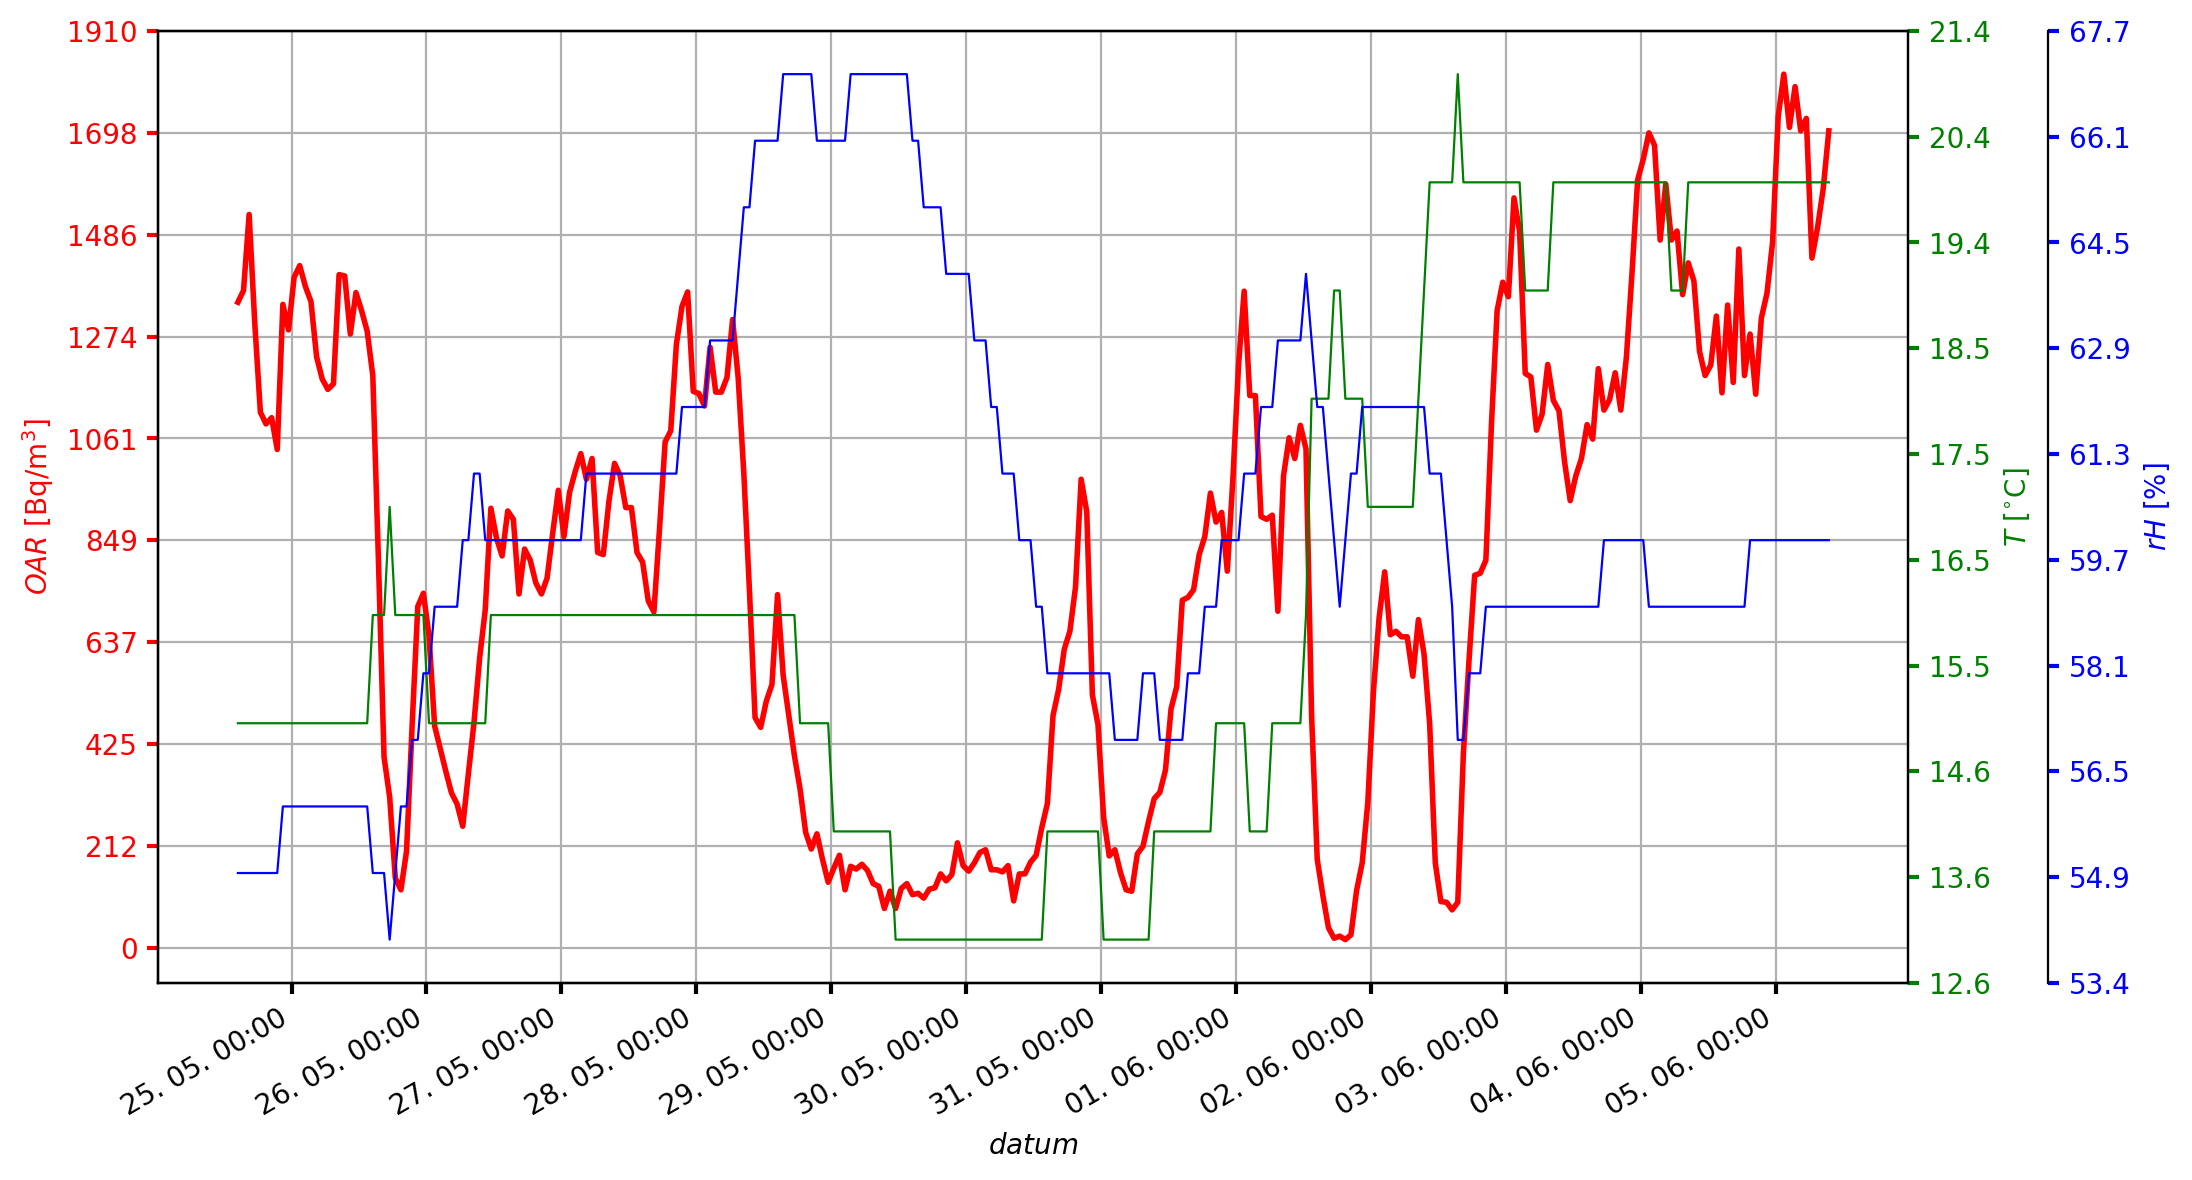
\includegraphics[height=0.8\textwidth, angle=-90, origin=c]{skala75/a2_1.png}
    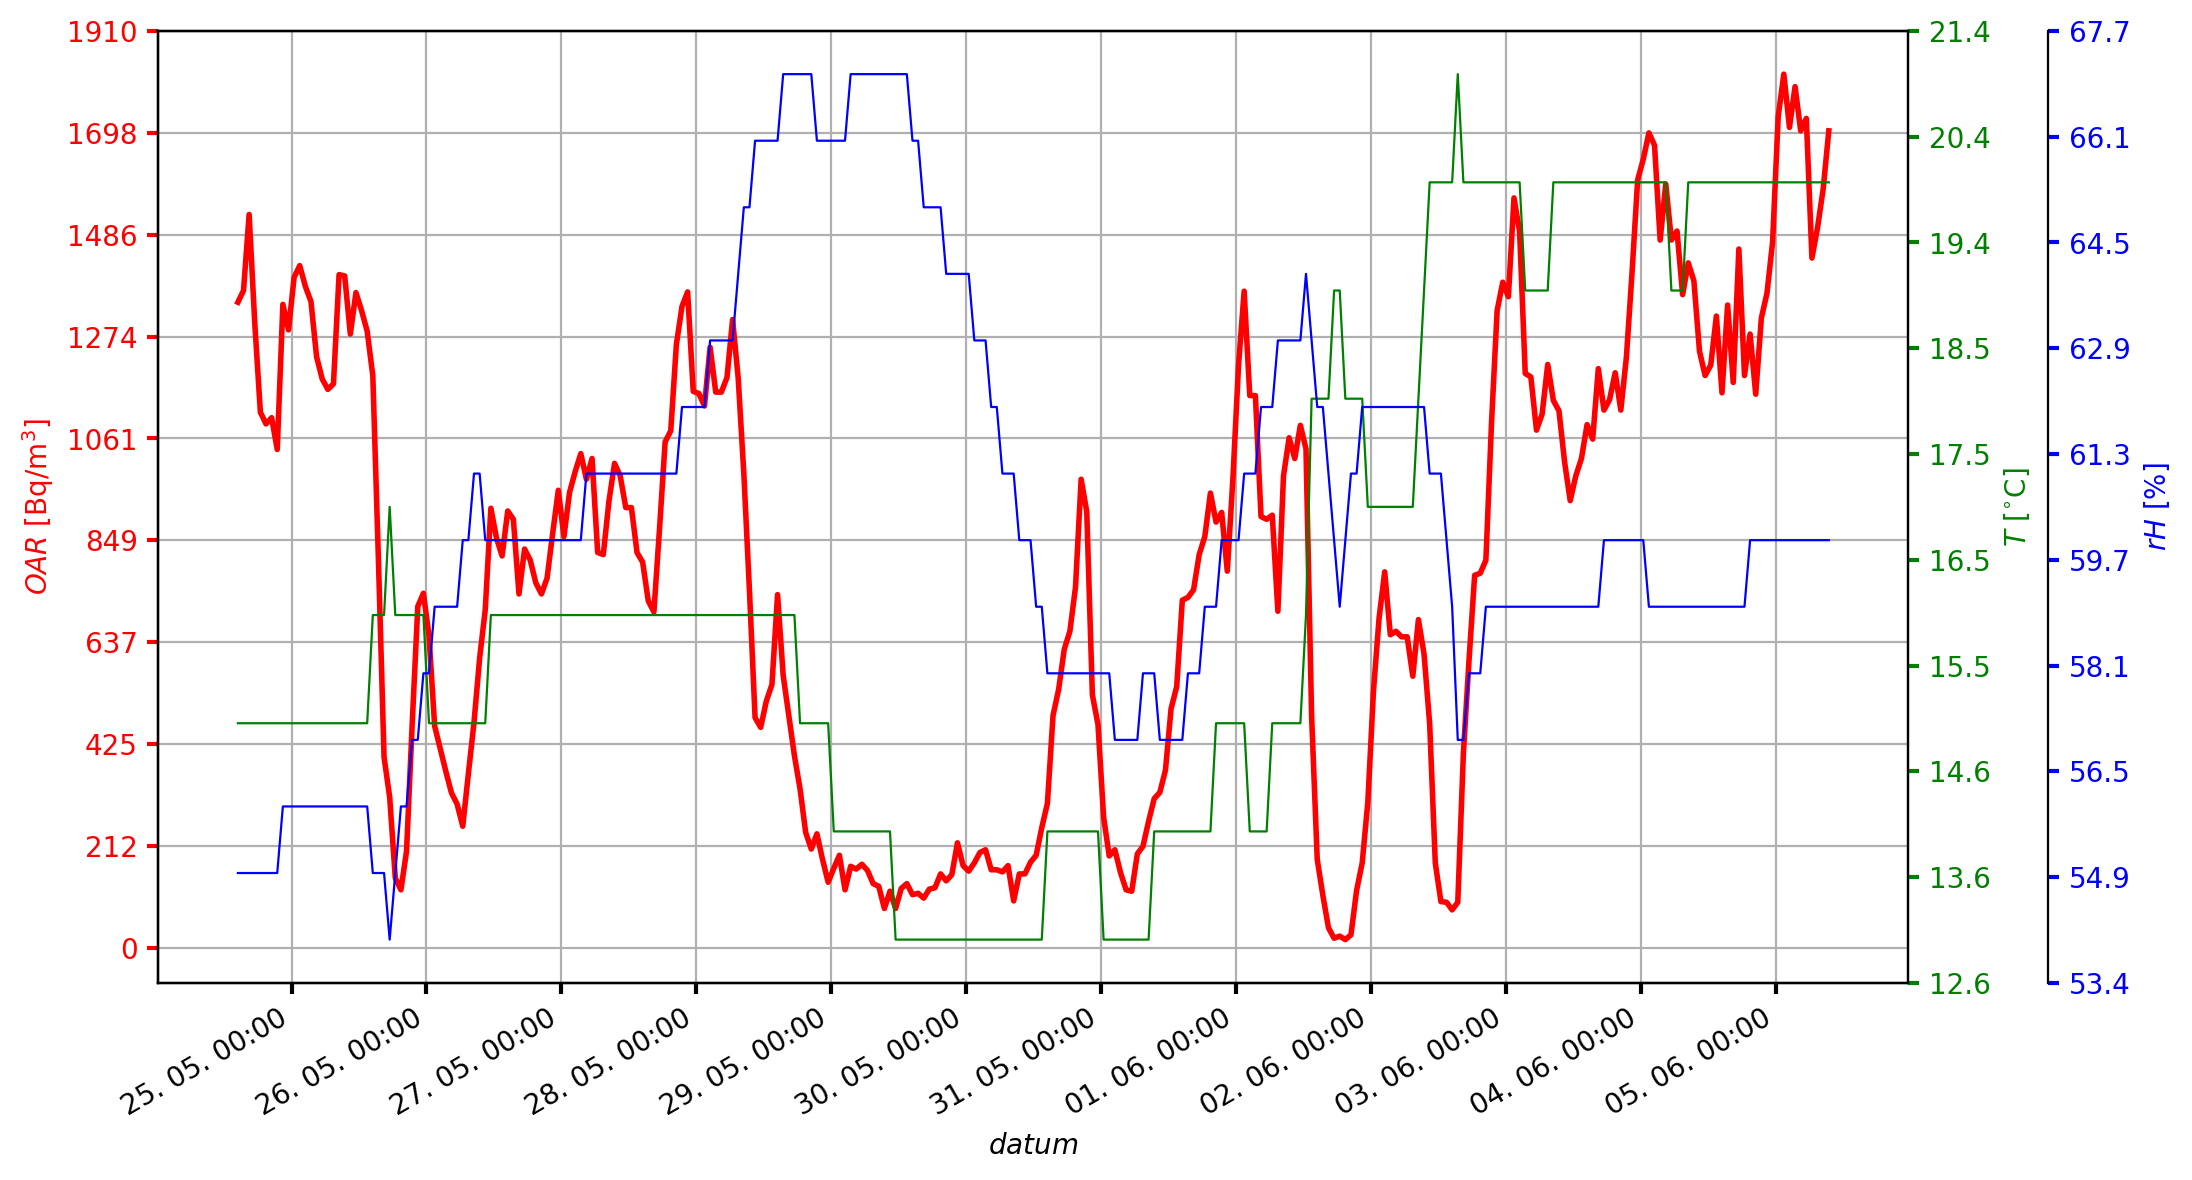
\includegraphics[width=1.1\textwidth]{skala75/a2_1.png}
    \caption{Data z TERA sondy č. 10, která byla umístěna v přízemí v kuchyni.}
    \label{fig:skala75_a2_1}
\end{figure}
\begin{figure}[H]
    \centering
    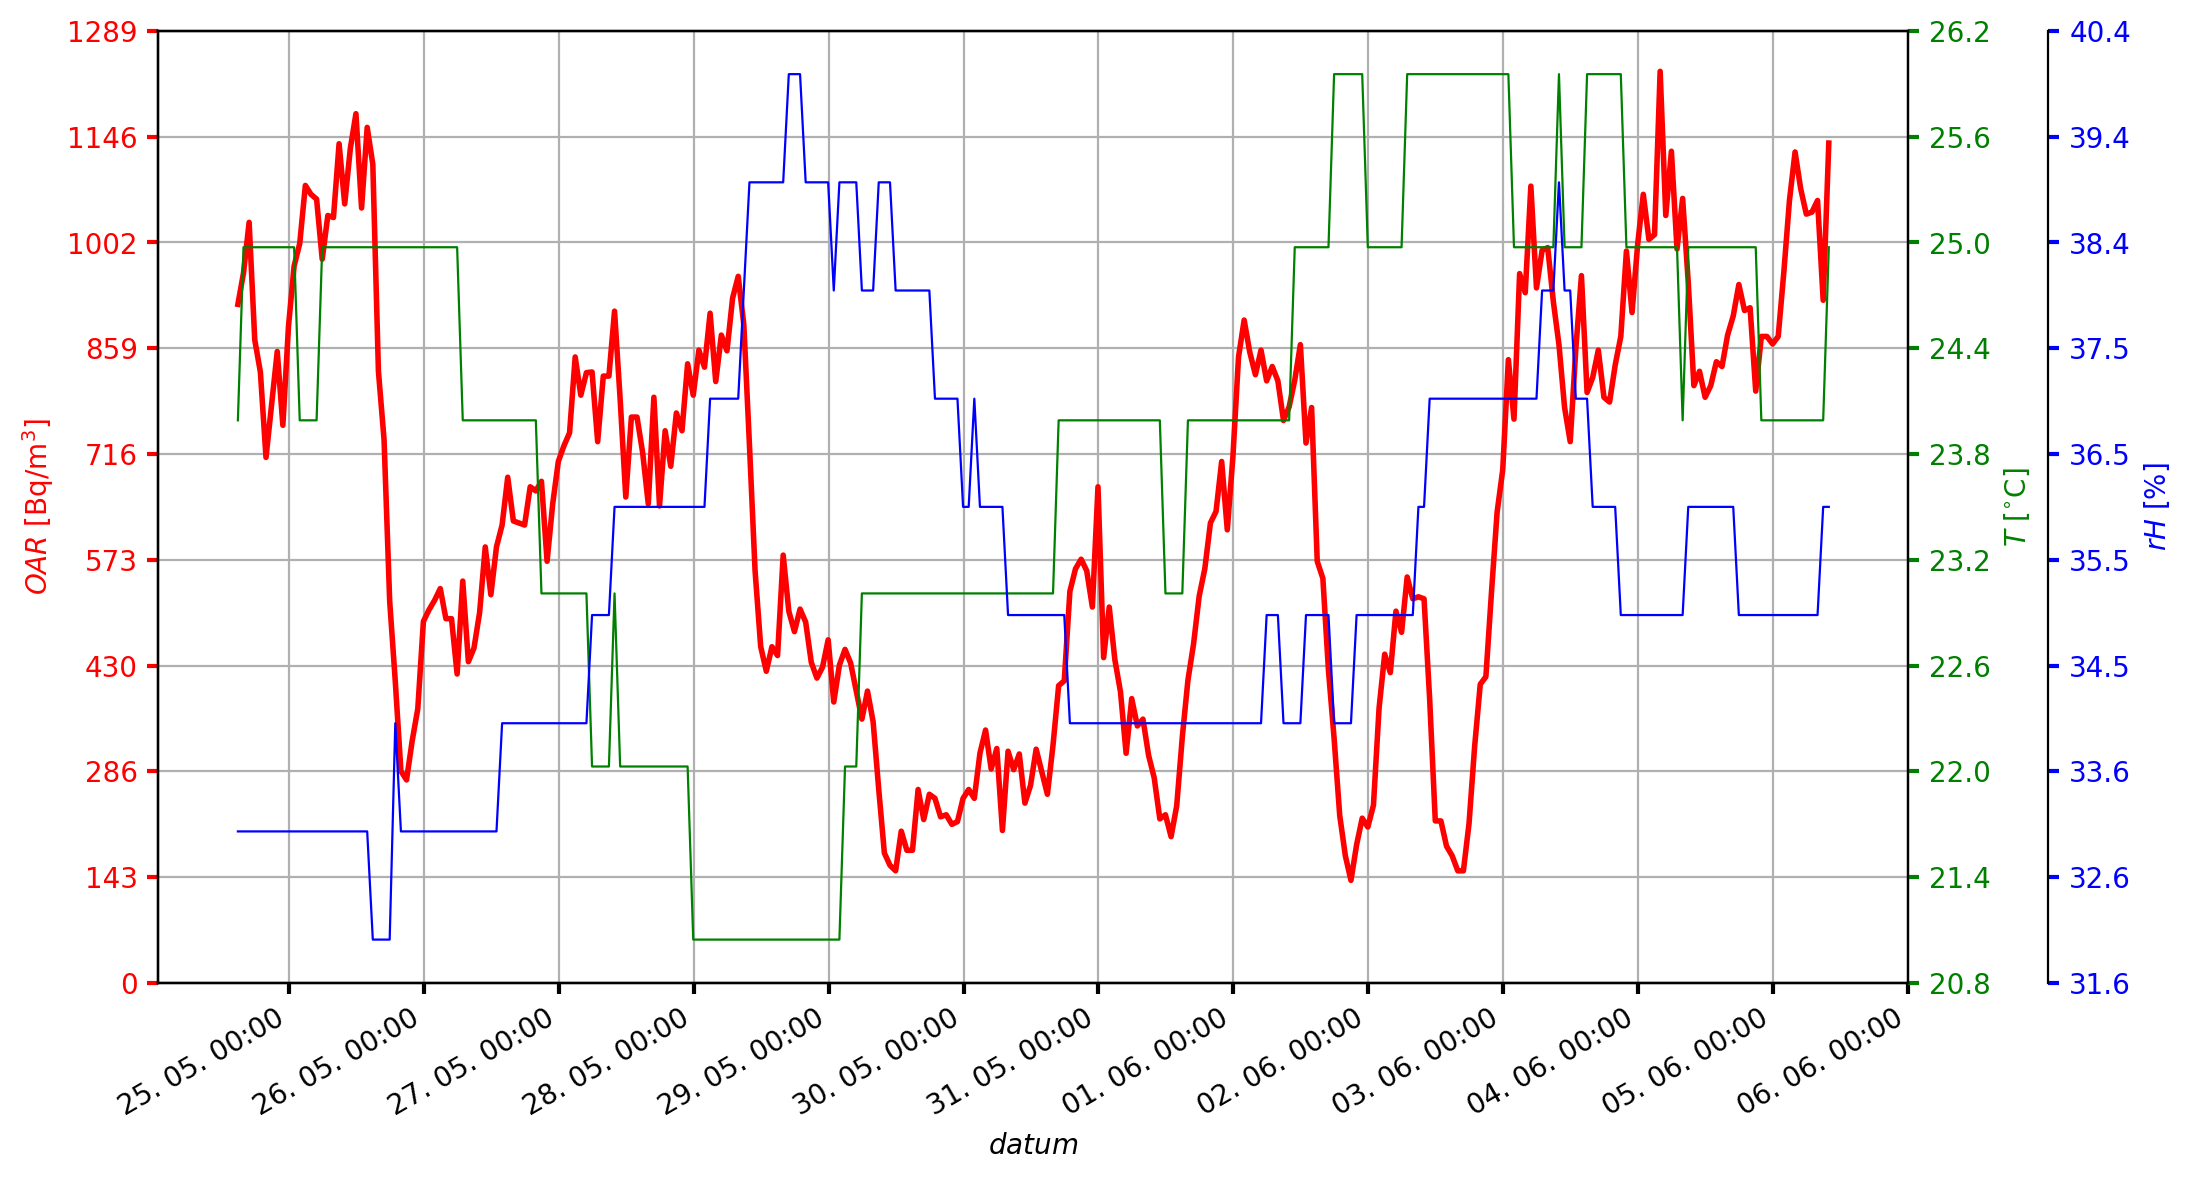
\includegraphics[width=1.1\textwidth]{skala75/a2_2.png}
    \caption{Data z TERA sondy č. 112, která byla umístěna v přízemí v ložnici.}
    \label{fig:skala75_a2_2}
\end{figure}
\begin{figure}[H]
    \centering
    \includegraphics[width=1.1\textwidth]{skala75/a3.png}
    \caption{Data z TERA sondy č. 88, která byla umístěna v prvním patře.}
    \label{fig:skala75_a3}
\end{figure}

\section{Přísuny radonu}

\begin{figure}[H]
    \centering
    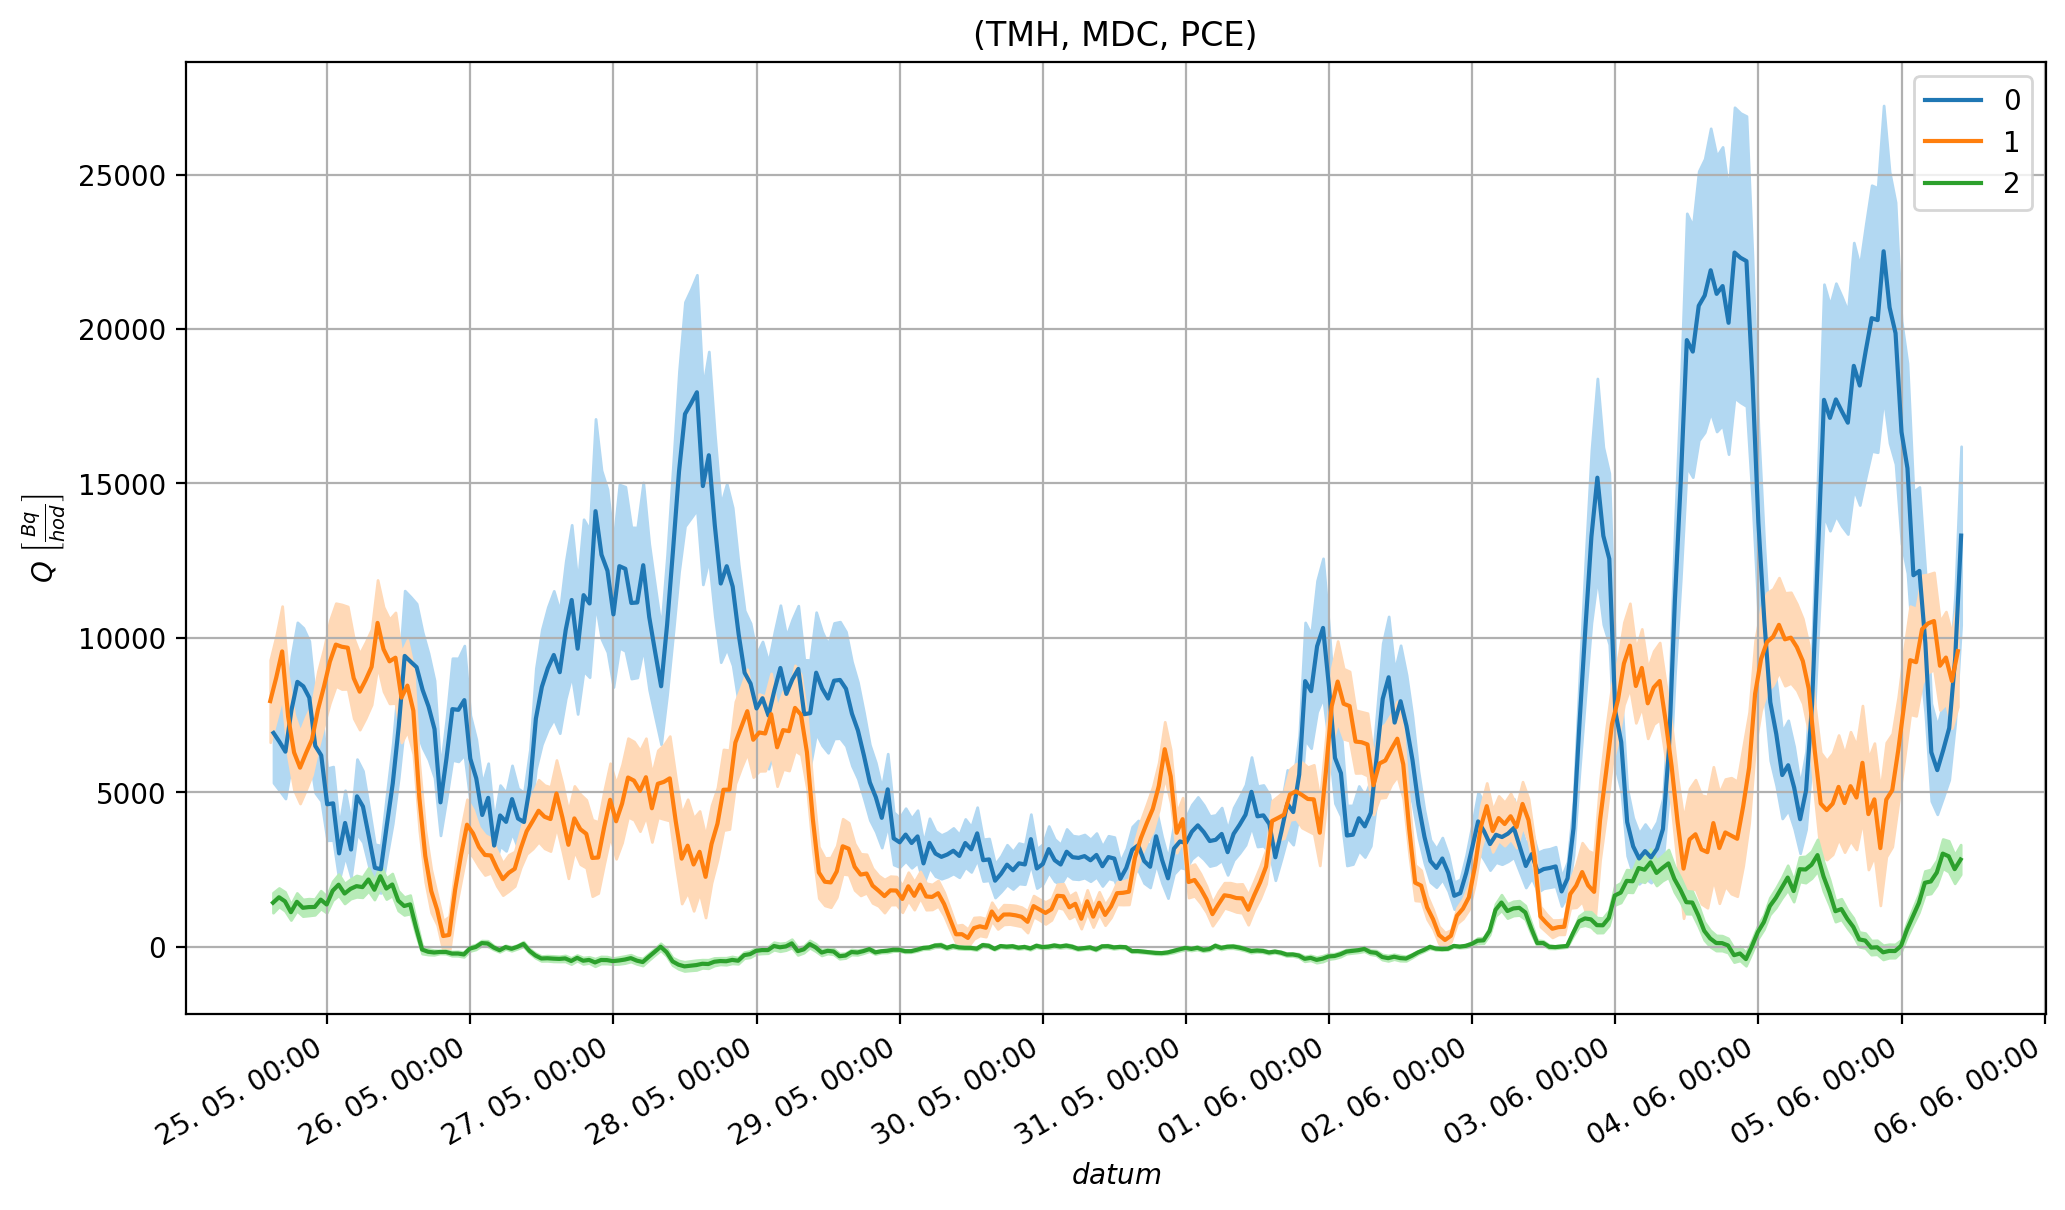
\includegraphics[width=\textwidth]{skala75/prisuny1.png}
    \caption{Určený časový vývoj přísunů radonu do jednotlivých podlaží. Nad obrázkem je uvedena kombinace tří použitých indikačních plynů. Oblasti označené zesvětlenou barvou značí nejistotu přísunů radonu při faktoru pokrytí $k=1$.}
    \label{fig:skala75_prisuny1}
\end{figure}
\begin{table}[H]
    \centering
    \caption{Statistiky vypočítaných přísunů radonu $Q$ do jednotlivých podlaží při stejné kombinaci použitých plynů jako v obr. nad touto tabulkou.}
    \label{tab:skala75_prisuny1}
    \begin{tabular}{lrrr}
\toprule
{} &  $Q_0$ $\left[\si{\frac{Bq}{m^3\cdot hod}}\right]$ &  $Q_1$ $\left[\si{\frac{Bq}{m^3\cdot hod}}\right]$ &  $Q_2$ $\left[\si{\frac{Bq}{m^3\cdot hod}}\right]$ \\
\midrule
count &                                                284 &                                                284 &                                                284 \\
mean  &                                                337 &                                                237 &                                                 19 \\
std   &                                                270 &                                                157 &                                                 84 \\
min   &                                                 15 &                                                -85 &                                               -269 \\
25%   &                                                137 &                                                102 &                                                -19 \\
50%   &                                                222 &                                                237 &                                                 -2 \\
75%   &                                                449 &                                                352 &                                                 29 \\
max   &                                               1161 &                                                891 &                                                371 \\
\bottomrule
\end{tabular}

\end{table}

\begin{figure}[H]
    \centering
    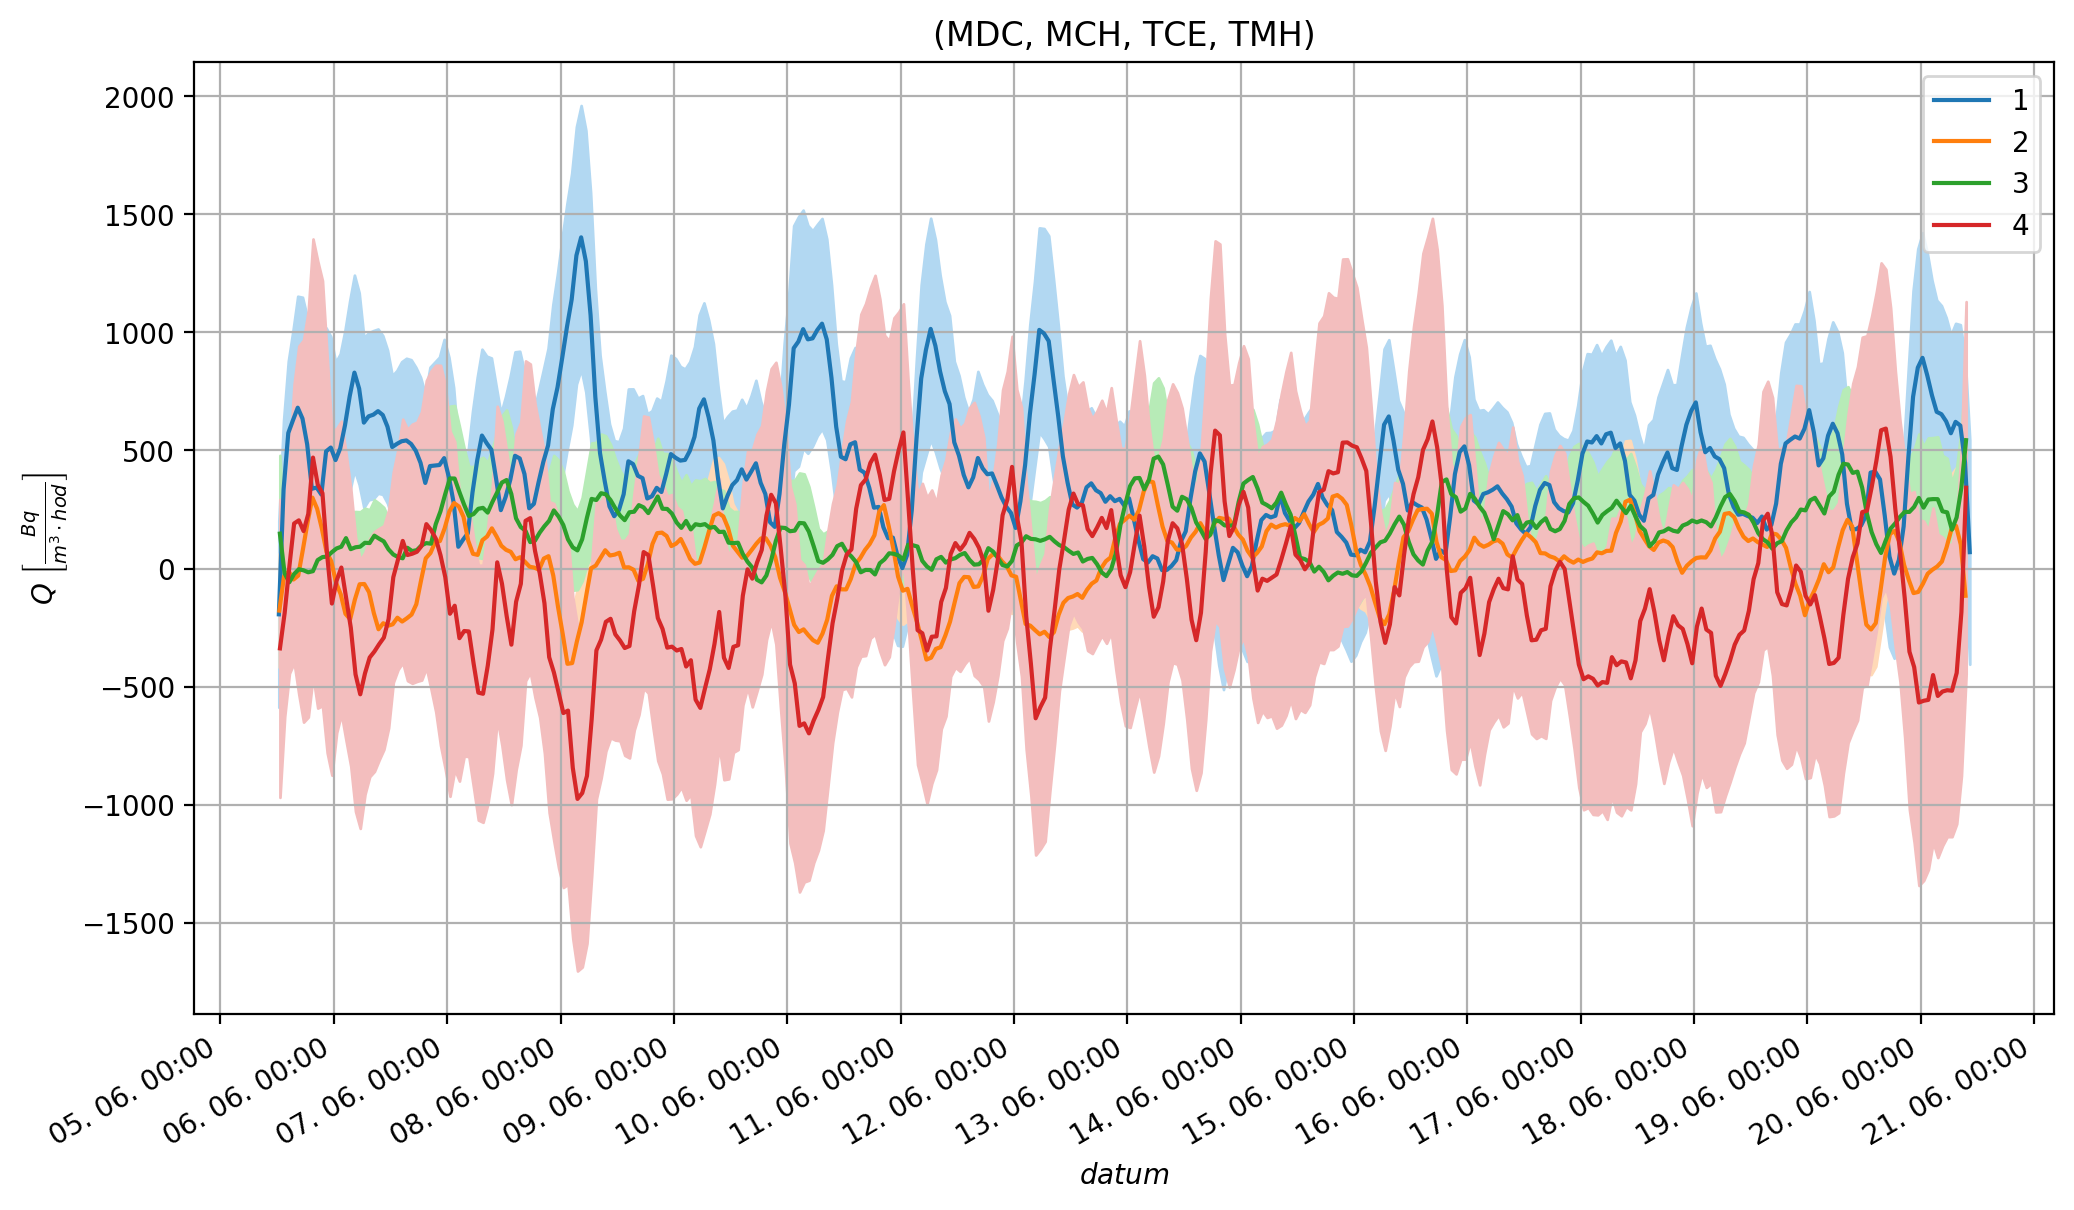
\includegraphics[width=\textwidth]{skala75/prisuny2.png}
    \caption{Určený časový vývoj přísunů radonu do jednotlivých podlaží. Nad obrázkem je uvedena kombinace tří použitých indikačních plynů. Oblasti označené zesvětlenou barvou značí nejistotu přísunů radonu při faktoru pokrytí $k=1$.}
    \label{fig:skala75_prisuny2}
\end{figure}
\begin{table}[H]
    \centering
    \caption{Statistiky vypočítaných přísunů radonu $Q$ do jednotlivých podlaží při stejné kombinaci použitých indikačních plynů jako v obr. nad touto tabulkou.}
    \label{tab:skala75_prisuny2}
    \begin{tabular}{lrrr}
\toprule
{} &  $Q_0$ $\left[\si{\frac{Bq}{hod}}\right]$ &  $Q_1$ $\left[\si{\frac{Bq}{hod}}\right]$ &  $Q_2$ $\left[\si{\frac{Bq}{hod}}\right]$ \\
\midrule
count &                                       284 &                                       284 &                                       284 \\
mean  &                                     12509 &                                     29052 &                                      4320 \\
%std   &                                     10164 &                                     15971 &                                     10993 \\
min   &                                     -1305 &                                      2758 &                                     -7217 \\
25\%   &                                      5053 &                                     13800 &                                     -2574 \\
50\%   &                                      8450 &                                     29570 &                                      -410 \\
75\%   &                                     16517 &                                     41212 &                                     10192 \\
max   &                                     42325 &                                     61230 &                                     36875 \\
\bottomrule
\end{tabular}

\end{table}

\begin{figure}[H]
    \centering
    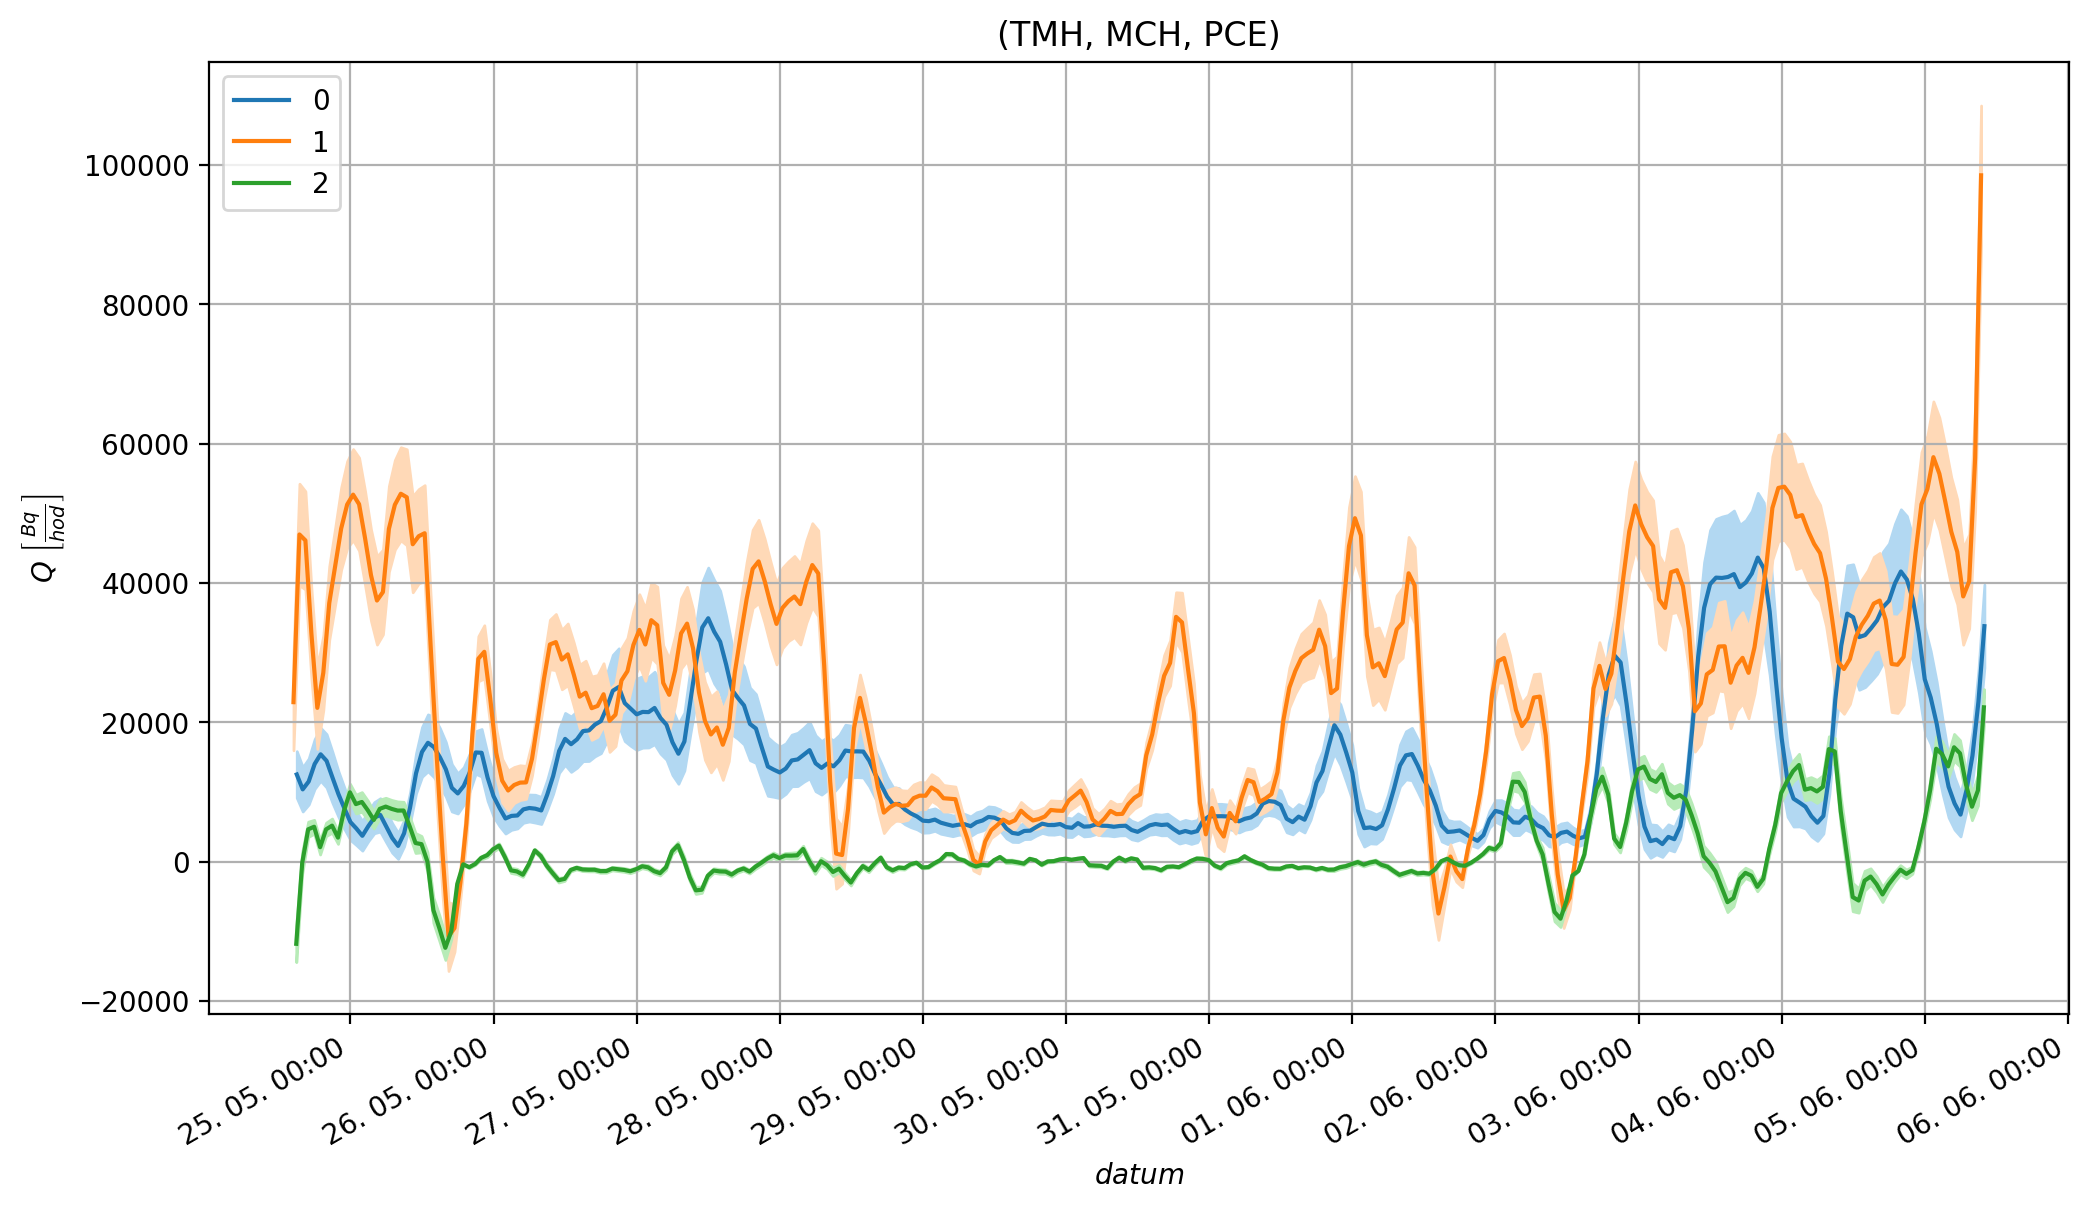
\includegraphics[width=\textwidth]{skala75/prisuny3.png}
    \caption{Určený časový vývoj přísunů radonu do jednotlivých podlaží. Nad obrázkem je uvedena kombinace tří použitých indikačních plynů. Oblasti označené zesvětlenou barvou značí nejistotu přísunů radonu při faktoru pokrytí $k=1$.}
    \label{fig:skala75_prisuny3}
\end{figure}
\begin{table}[H]
    \centering
    \caption{Statistiky vypočítaných přísunů radonu $Q$ do jednotlivých podlaží při stejné kombinaci použitých indikačních plynů jako v obr. nad touto tabulkou.}
    \label{tab:skala75_prisuny3}
    \begin{tabular}{lrrr}
\toprule
{} &  $Q_0$ $\left[\si{\frac{Bq}{hod}}\right]$ &  $Q_1$ $\left[\si{\frac{Bq}{hod}}\right]$ &  $Q_2$ $\left[\si{\frac{Bq}{hod}}\right]$ \\
\midrule
count &                                       284 &                                       284 &                                       284 \\
mean  &                                     13429 &                                     24771 &                                      1333 \\
std   &                                     10114 &                                     14050 &                                      2973 \\
min   &                                      2390 &                                      2315 &                                     -1709 \\
25%   &                                      5647 &                                     11702 &                                      -535 \\
50%   &                                      9781 &                                     24454 &                                       -12 \\
75%   &                                     17323 &                                     35419 &                                      2907 \\
max   &                                     42770 &                                     53869 &                                     10103 \\
\bottomrule
\end{tabular}

\end{table}

\begin{figure}[H]
    \centering
    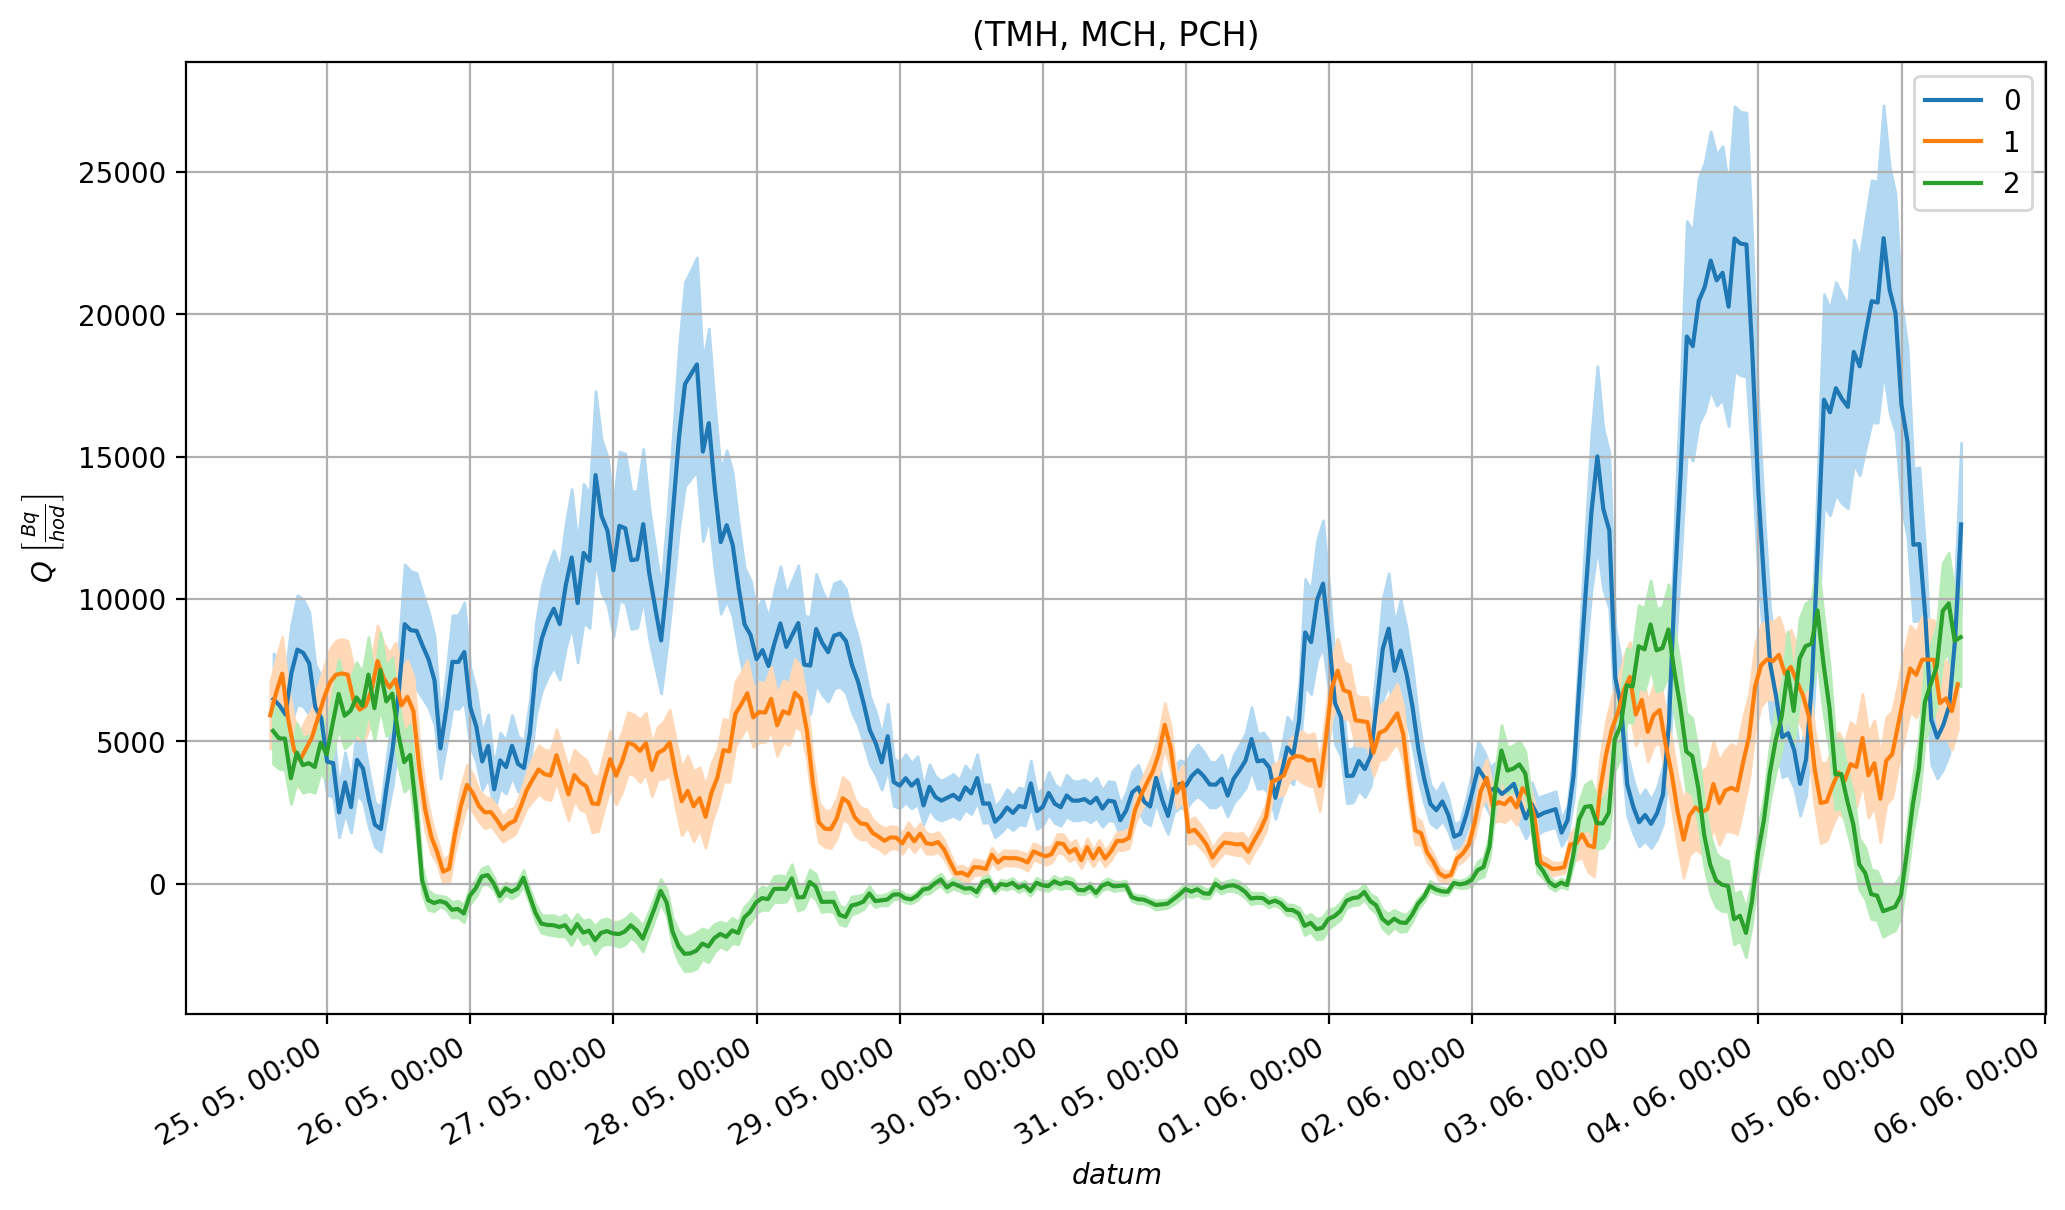
\includegraphics[width=\textwidth]{skala75/prisuny4.png}
    \caption{Určený časový vývoj přísunů radonu do jednotlivých podlaží. Nad obrázkem je uvedena kombinace tří použitých indikačních plynů. Oblasti označené zesvětlenou barvou značí nejistotu přísunů radonu při faktoru pokrytí $k=1$.}
    \label{fig:skala75_prisuny4}
\end{figure}
\begin{table}[H]
    \centering
    \caption{Statistiky vypočítaných přísunů radonu $Q$ do jednotlivých podlaží při stejné kombinaci použitých indikačních plynů jako v obr. nad touto tabulkou.}
    \label{tab:skala75_prisuny4}
    \begin{tabular}{lrrr}
\toprule
{} &  $Q_0$ $\left[\si{\frac{Bq}{hod}}\right]$ &  $Q_1$ $\left[\si{\frac{Bq}{hod}}\right]$ &  $Q_2$ $\left[\si{\frac{Bq}{hod}}\right]$ \\
\midrule
count &                                       284 &                                       284 &                                       284 \\
mean  &                                     12921 &                                     24194 &                                      4807 \\
%std   &                                     10215 &                                     13297 &                                     11131 \\
min   &                                      -501 &                                      2305 &                                     -6720 \\
25\%   &                                      5361 &                                     11493 &                                     -2236 \\
50\%   &                                      8950 &                                     24629 &                                      -191 \\
75\%   &                                     17045 &                                     34319 &                                     10881 \\
max   &                                     42783 &                                     50985 &                                     37529 \\
\bottomrule
\end{tabular}

\end{table}

\begin{figure}[H]
    \centering
    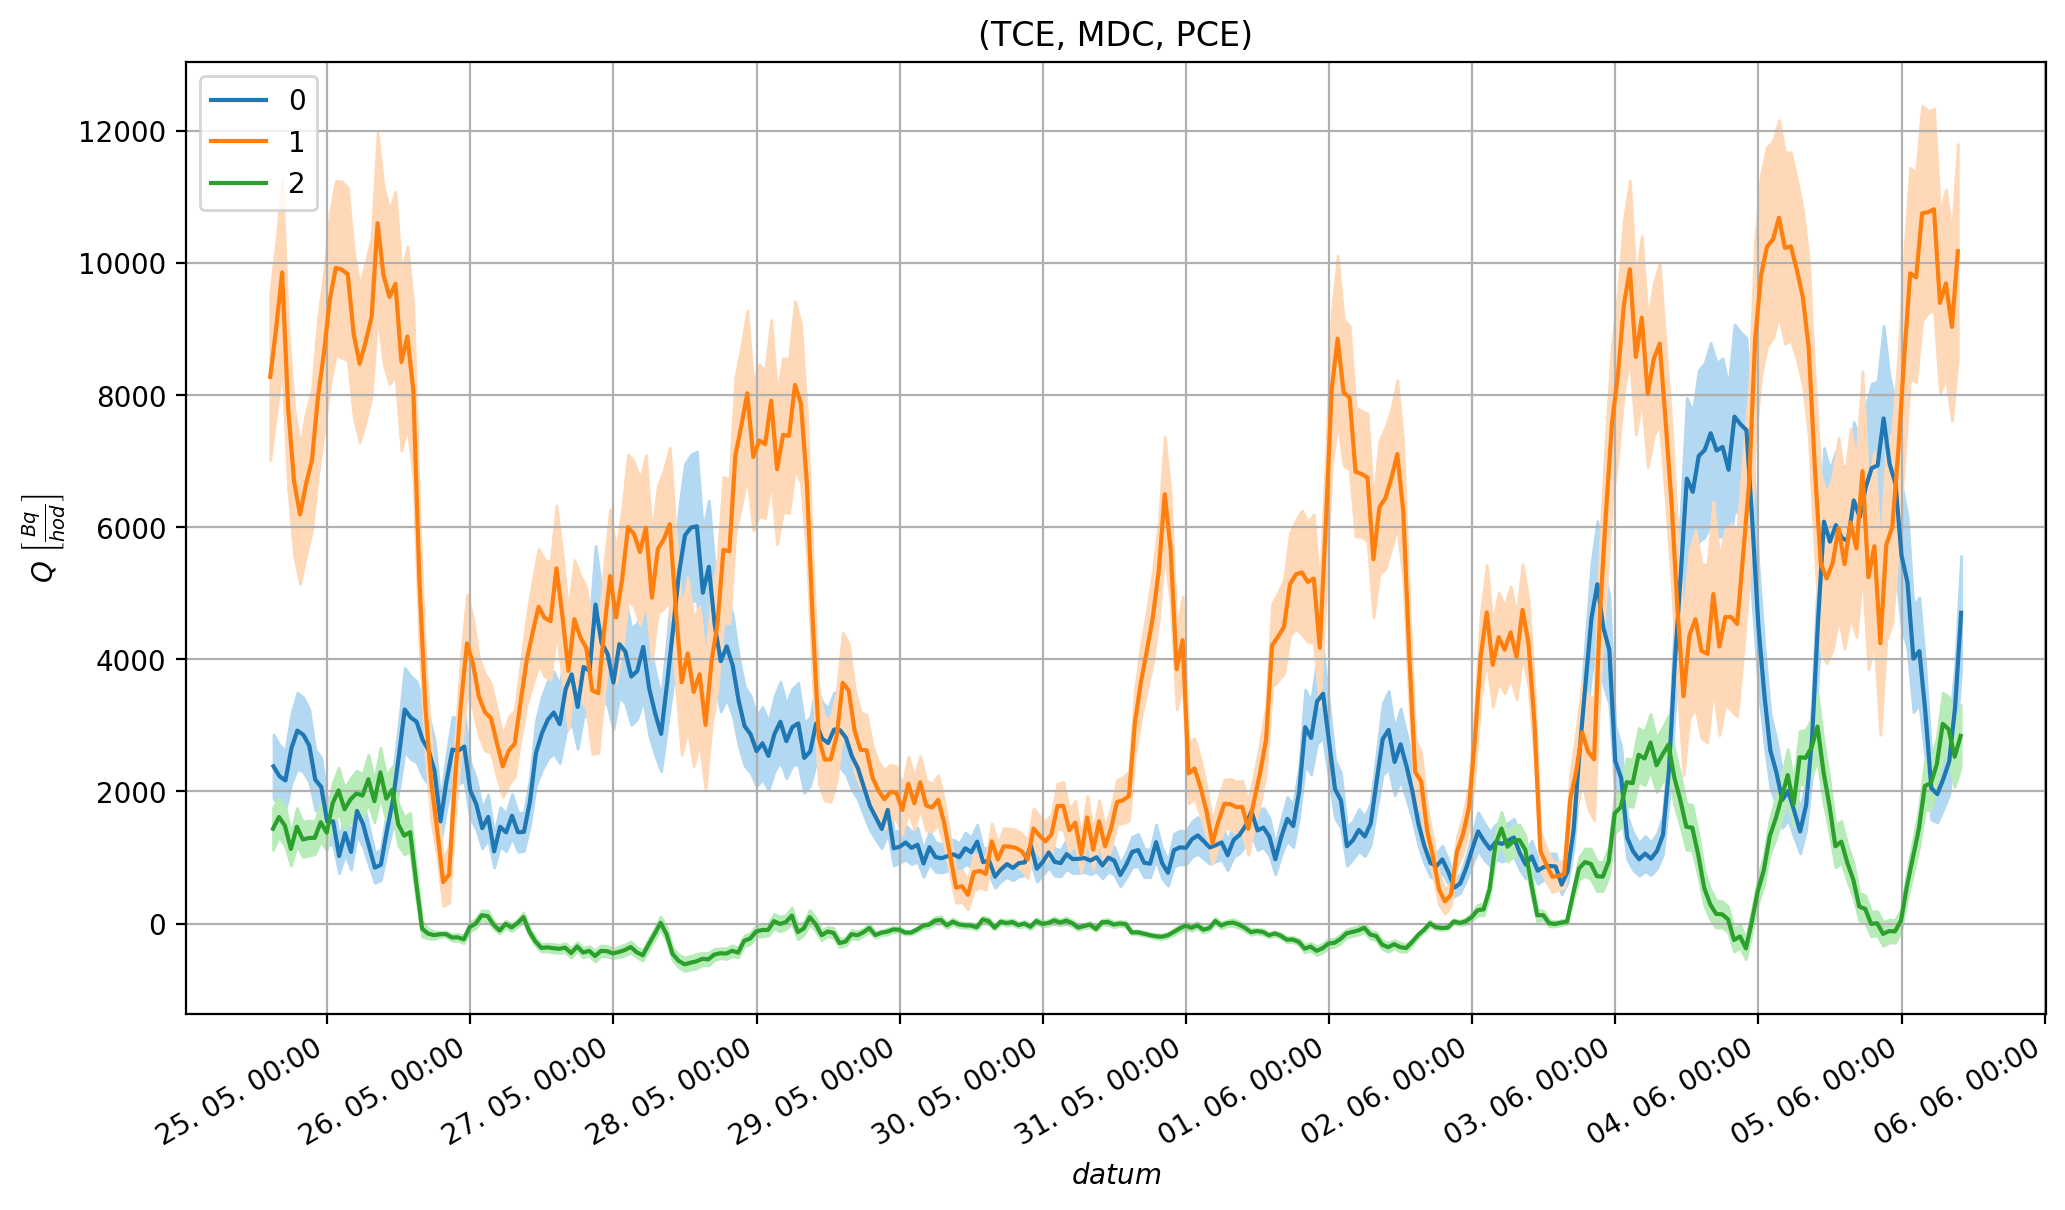
\includegraphics[width=\textwidth]{skala75/prisuny5.png}
    \caption{Určený časový vývoj přísunů radonu do jednotlivých podlaží. Nad obrázkem je uvedena kombinace tří použitých indikačních plynů. Oblasti označené zesvětlenou barvou značí nejistotu přísunů radonu při faktoru pokrytí $k=1$.}
    \label{fig:skala75_prisuny5}
\end{figure}
\begin{table}[H]
    \centering
    \caption{Statistiky vypočítaných přísunů radonu $Q$ do jednotlivých podlaží při stejné kombinaci použitých indikačních plynů jako v obr. nad touto tabulkou.}
    \label{tab:skala75_prisuny5}
    \begin{tabular}{lrrr}
\toprule
{} &  $Q_0$ $\left[\si{\frac{Bq}{m^3\cdot hod}}\right]$ &  $Q_1$ $\left[\si{\frac{Bq}{m^3\cdot hod}}\right]$ &  $Q_2$ $\left[\si{\frac{Bq}{m^3\cdot hod}}\right]$ \\
\midrule
count &                                                284 &                                                284 &                                                284 \\
mean  &                                                113 &                                                250 &                                                 19 \\
%std   &                                                116 &                                                160 &                                                 85 \\
min   &                                                -85 &                                                -78 &                                               -269 \\
25\%   &                                                 37 &                                                111 &                                                -20 \\
50\%   &                                                 74 &                                                255 &                                                 -2 \\
75\%   &                                                161 &                                                369 &                                                 29 \\
max   &                                                528 &                                                913 &                                                371 \\
\bottomrule
\end{tabular}

\end{table}

\begin{figure}[H]
    \centering
    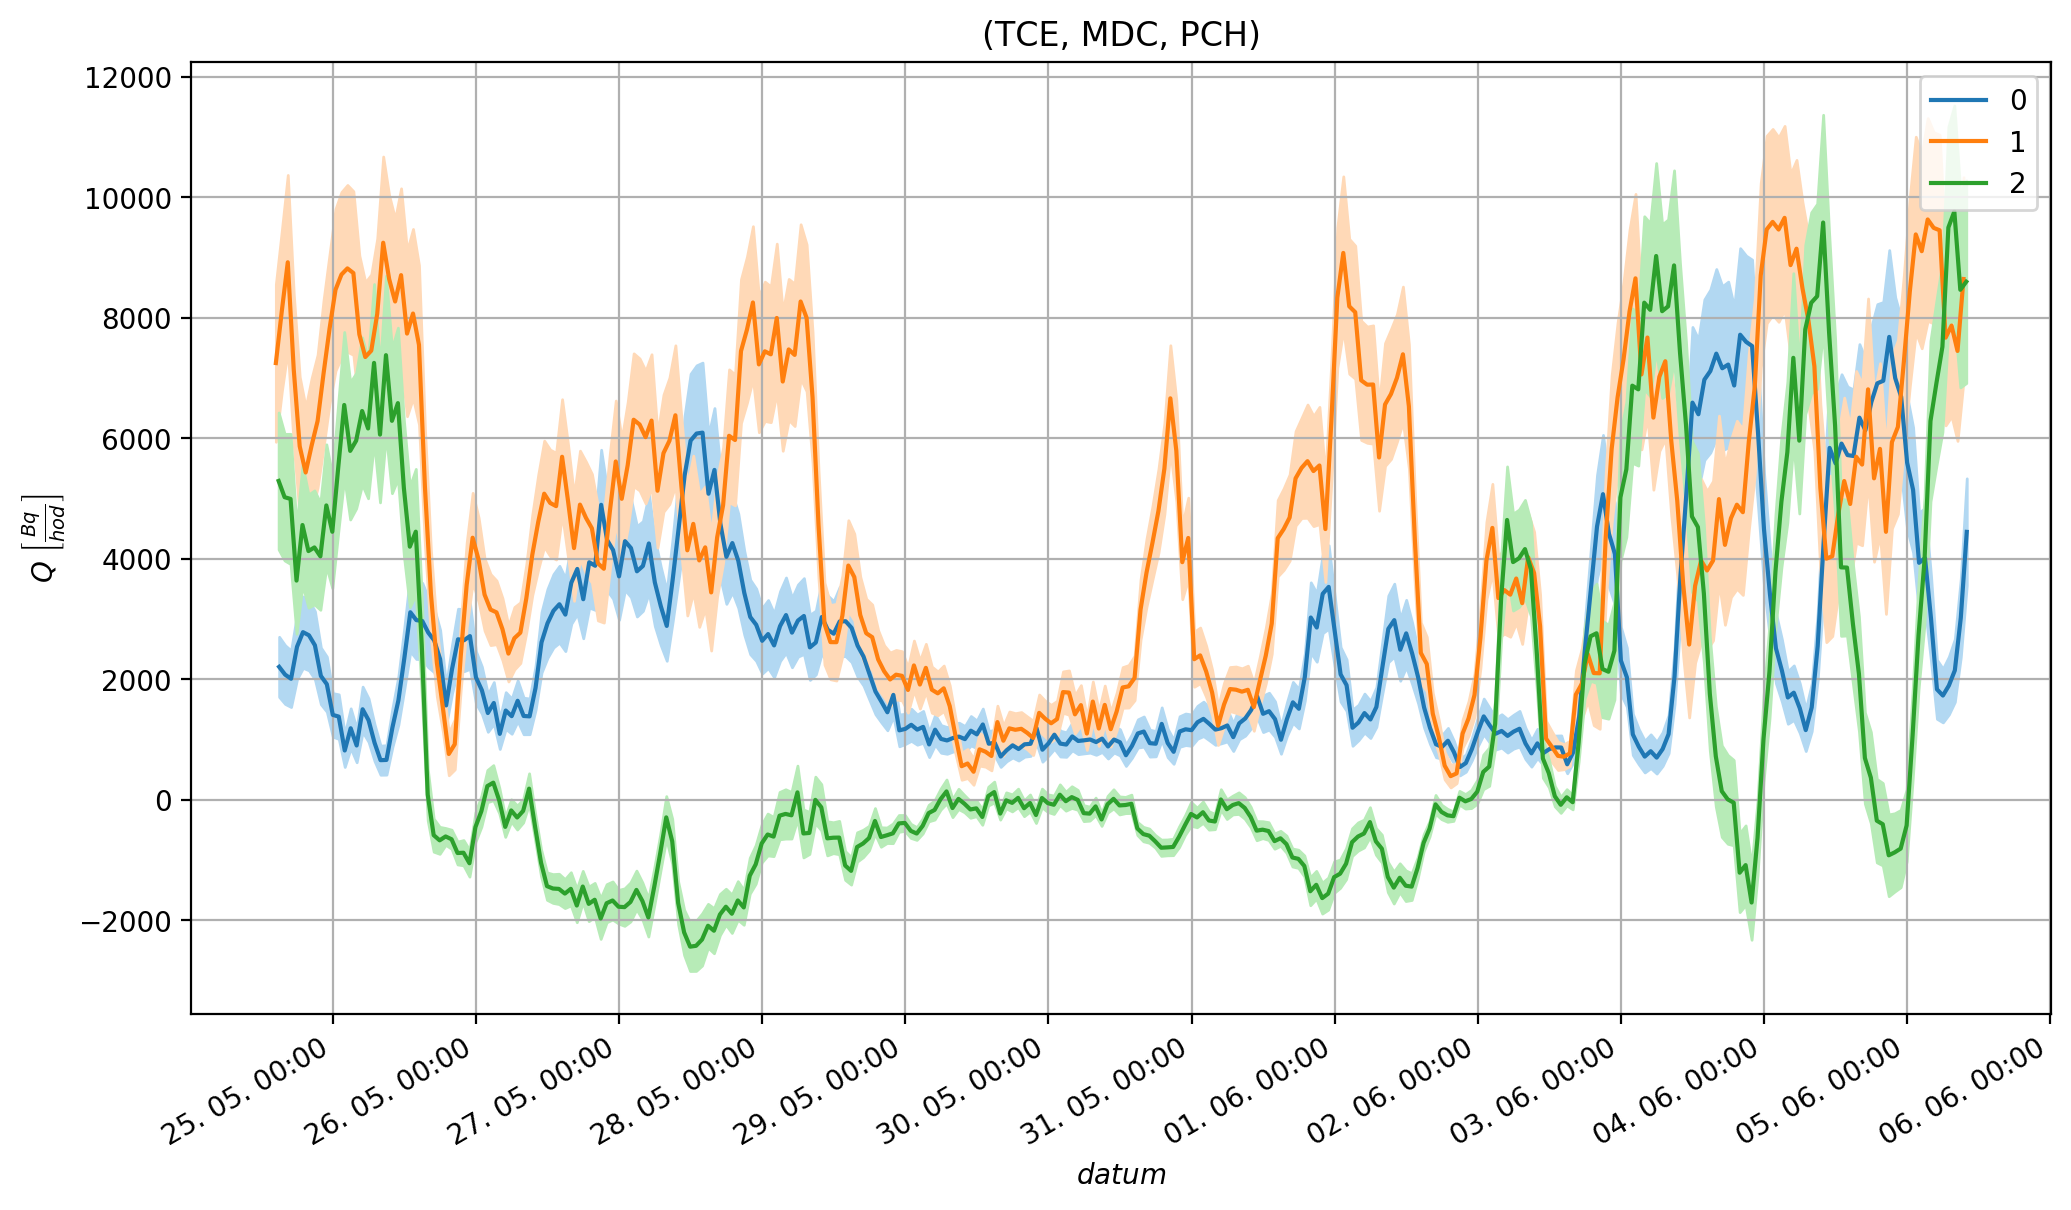
\includegraphics[width=\textwidth]{skala75/prisuny6.png}
    \caption{Určený časový vývoj přísunů radonu do jednotlivých podlaží. Nad obrázkem je uvedena kombinace tří použitých indikačních plynů. Oblasti označené zesvětlenou barvou značí nejistotu přísunů radonu při faktoru pokrytí $k=1$.}
    \label{fig:skala75_prisuny6}
\end{figure}
\begin{table}[H]
    \centering
    \caption{Statistiky vypočítaných přísunů radonu $Q$ do jednotlivých podlaží při stejné kombinaci použitých indikačních plynů jako v obr. nad touto tabulkou.}
    \label{tab:skala75_prisuny6}
    \begin{tabular}{lrrr}
\toprule
{} &  $Q_0$ $\left[\si{\frac{Bq}{hod}}\right]$ &  $Q_1$ $\left[\si{\frac{Bq}{hod}}\right]$ &  $Q_2$ $\left[\si{\frac{Bq}{hod}}\right]$ \\
\midrule
count &                                       284 &                                       284 &                                       284 \\
mean  &                                      4233 &                                     30807 &                                      4359 \\
%std   &                                      4526 &                                     19577 &                                     12339 \\
min   &                                     -4010 &                                    -10346 &                                    -16011 \\
25\%   &                                      1203 &                                     13494 &                                     -3348 \\
50\%   &                                      2855 &                                     31079 &                                      -669 \\
75\%   &                                      6299 &                                     45500 &                                      8645 \\
max   &                                     19350 &                                    110431 &                                     49402 \\
\bottomrule
\end{tabular}

\end{table}

\begin{figure}[H]
    \centering
    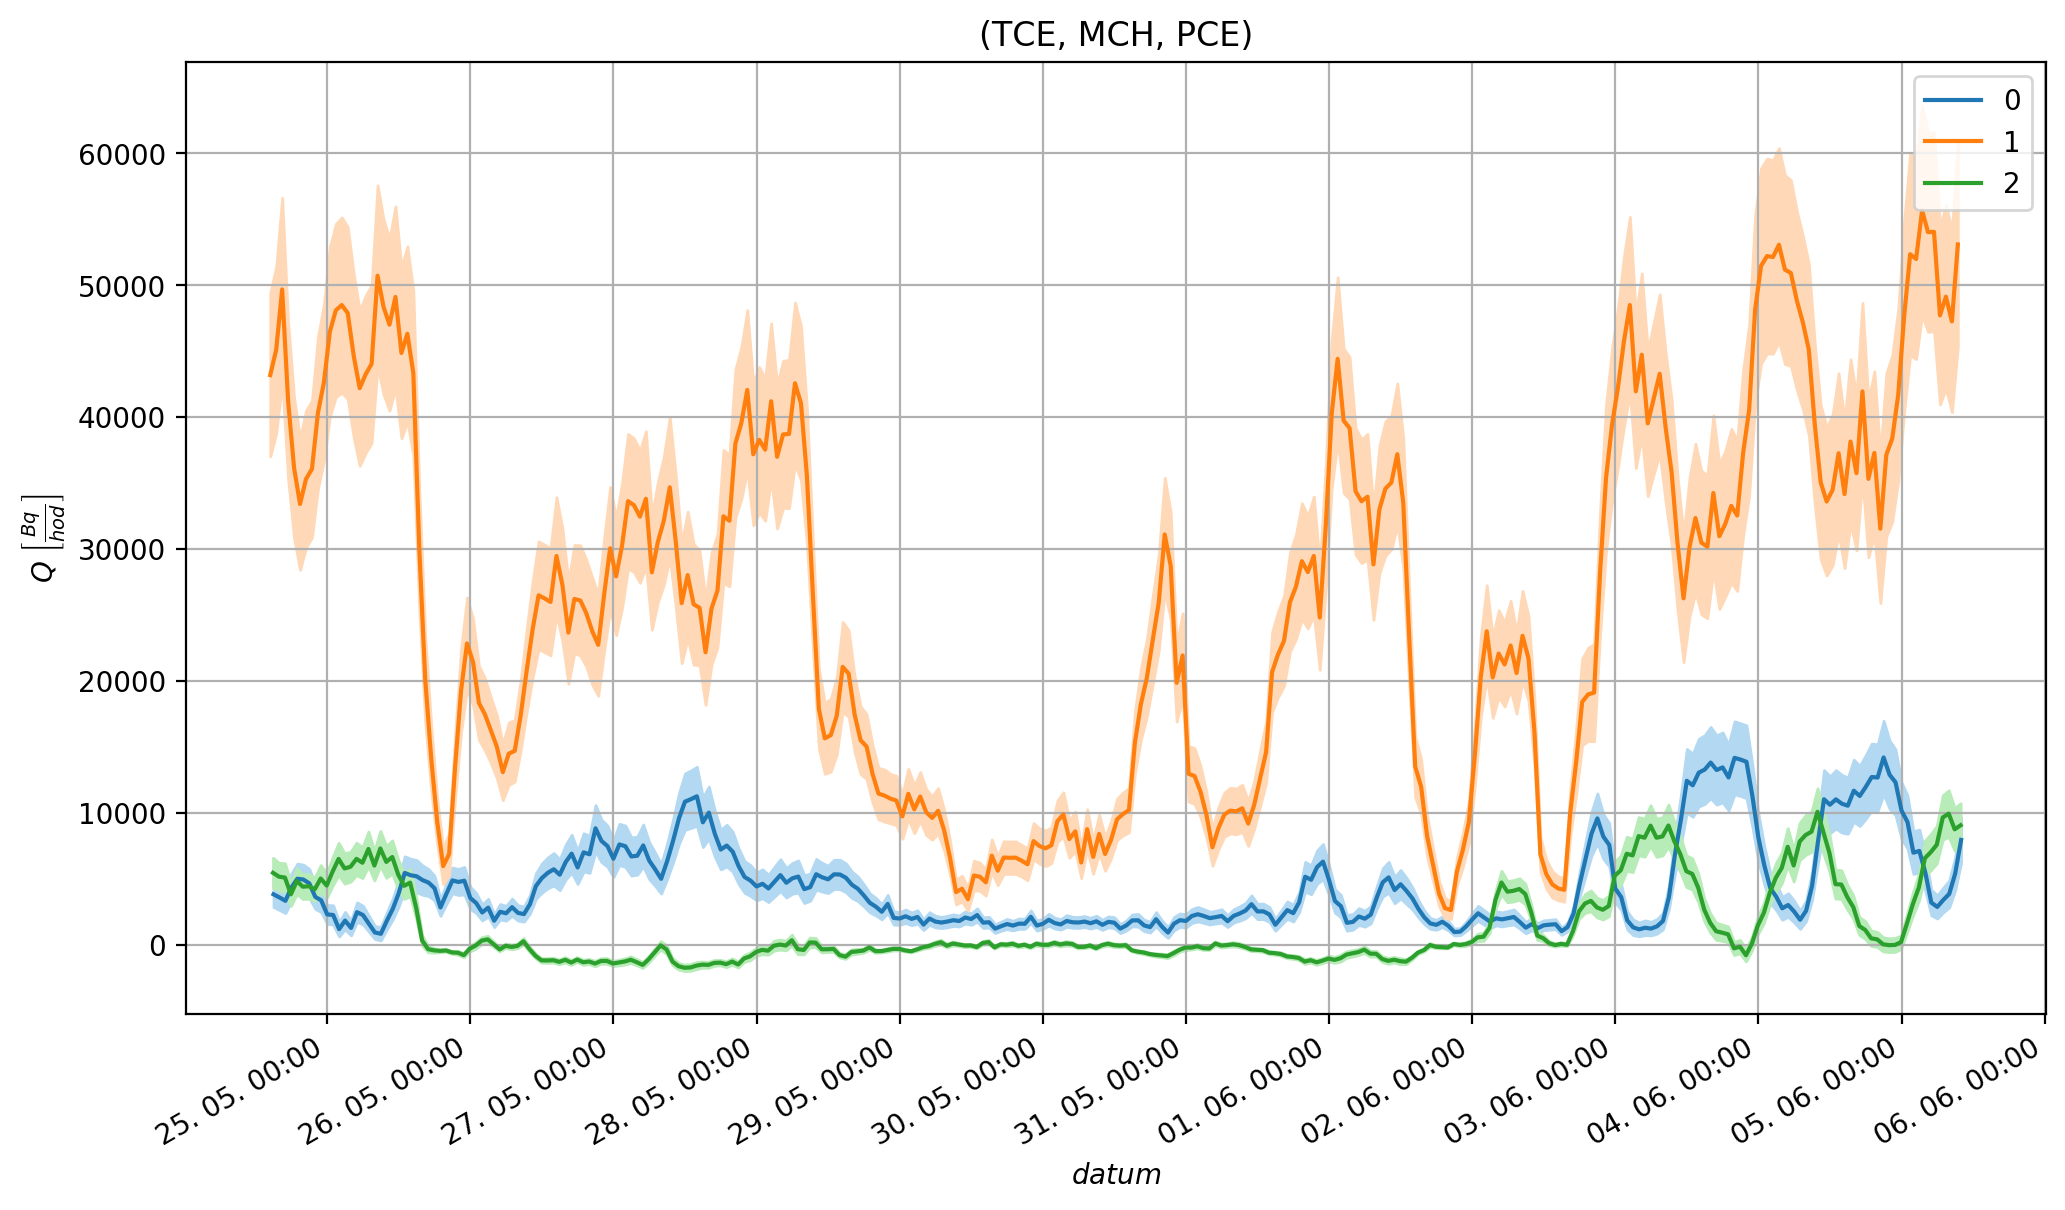
\includegraphics[width=\textwidth]{skala75/prisuny7.png}
    \caption{Určený časový vývoj přísunů radonu do jednotlivých podlaží. Nad obrázkem je uvedena kombinace tří použitých indikačních plynů. Oblasti označené zesvětlenou barvou značí nejistotu přísunů radonu při faktoru pokrytí $k=1$.}
    \label{fig:skala75_prisuny7}
\end{figure}
\begin{table}[H]
    \centering
    \caption{Statistiky vypočítaných přísunů radonu $Q$ do jednotlivých podlaží při stejné kombinaci použitých indikačních plynů jako v obr. nad touto tabulkou.}
    \label{tab:skala75_prisuny7}
    \begin{tabular}{lrrr}
\toprule
{} &  $Q_0$ $\left[\si{\frac{Bq}{hod}}\right]$ &  $Q_1$ $\left[\si{\frac{Bq}{hod}}\right]$ &  $Q_2$ $\left[\si{\frac{Bq}{hod}}\right]$ \\
\midrule
count &                                       284 &                                       284 &                                       284 \\
mean  &                                      4466 &                                     26182 &                                      1325 \\
%std   &                                      3357 &                                     14388 &                                      2973 \\
min   &                                       847 &                                      2646 &                                     -1726 \\
25\%   &                                      1868 &                                     12472 &                                      -540 \\
50\%   &                                      3228 &                                     26241 &                                       -15 \\
75\%   &                                      5735 &                                     37368 &                                      2890 \\
max   &                                     14210 &                                     55660 &                                     10091 \\
\bottomrule
\end{tabular}

\end{table}

\begin{figure}[H]
    \centering
    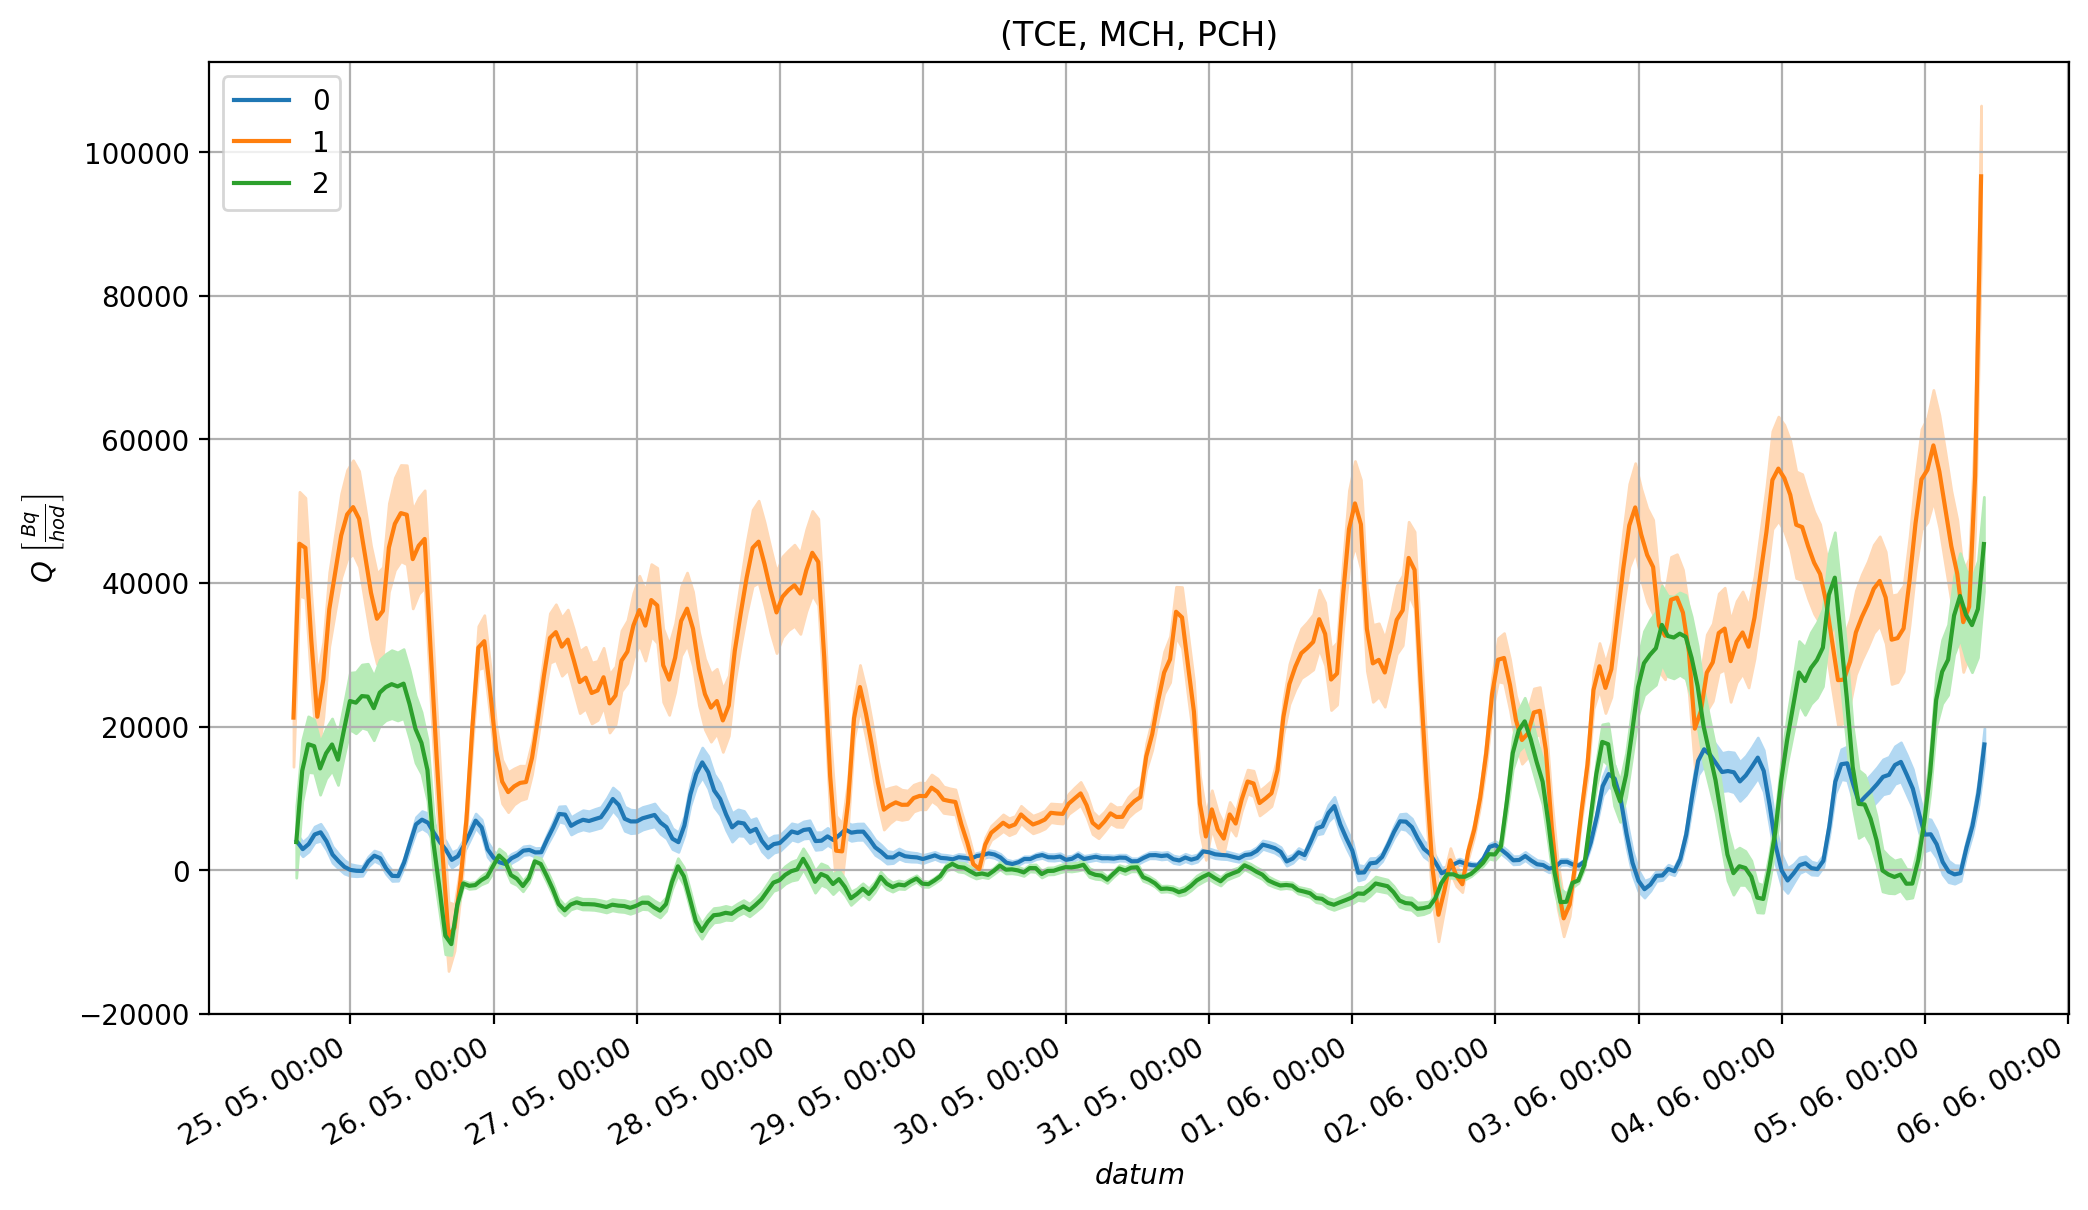
\includegraphics[width=\textwidth]{skala75/prisuny8.png}
    \caption{Určený časový vývoj přísunů radonu do jednotlivých podlaží. Nad obrázkem je uvedena kombinace tří použitých indikačních plynů. Oblasti označené zesvětlenou barvou značí nejistotu přísunů radonu při faktoru pokrytí $k=1$.}
    \label{fig:skala75_prisuny8}
\end{figure}
\begin{table}[H]
    \centering
    \caption{Statistiky vypočítaných přísunů radonu $Q$ do jednotlivých podlaží při stejné kombinaci použitých indikačních plynů jako v obr. nad touto tabulkou.}
    \label{tab:skala75_prisuny8}
    \begin{tabular}{lrrr}
\toprule
{} &  $Q_0$ $\left[\si{\frac{Bq}{m^3\cdot hod}}\right]$ &  $Q_1$ $\left[\si{\frac{Bq}{m^3\cdot hod}}\right]$ &  $Q_2$ $\left[\si{\frac{Bq}{m^3\cdot hod}}\right]$ \\
\midrule
count &                                                284 &                                                284 &                                                284 \\
mean  &                                               2536 &                                               3929 &                                               1148 \\
std   &                                               1795 &                                               2200 &                                               3007 \\
min   &                                                545 &                                                337 &                                              -2379 \\
25\%   &                                               1145 &                                               1866 &                                               -643 \\
50\%   &                                               1934 &                                               3842 &                                               -135 \\
75\%   &                                               3243 &                                               5850 &                                               2588 \\
max   &                                               7736 &                                               8235 &                                               9876 \\
\bottomrule
\end{tabular}

\end{table}

\chapter{Přílohy k objektu Hálková 980, Humpolec}\label{navesti:priloha_humpolec980}

\section{Schéma objektu}

\section{Naměřené vývoje OAR, teplot a relativní vlhkosti vzduchu}


\chapter{Přílohy k objektu Anglická 574, Dobřichovice}\label{navesti:priloha_anglicka574}

\section{Fotografie a schéma objektu}
\begin{figure}[ht]
    \centering
    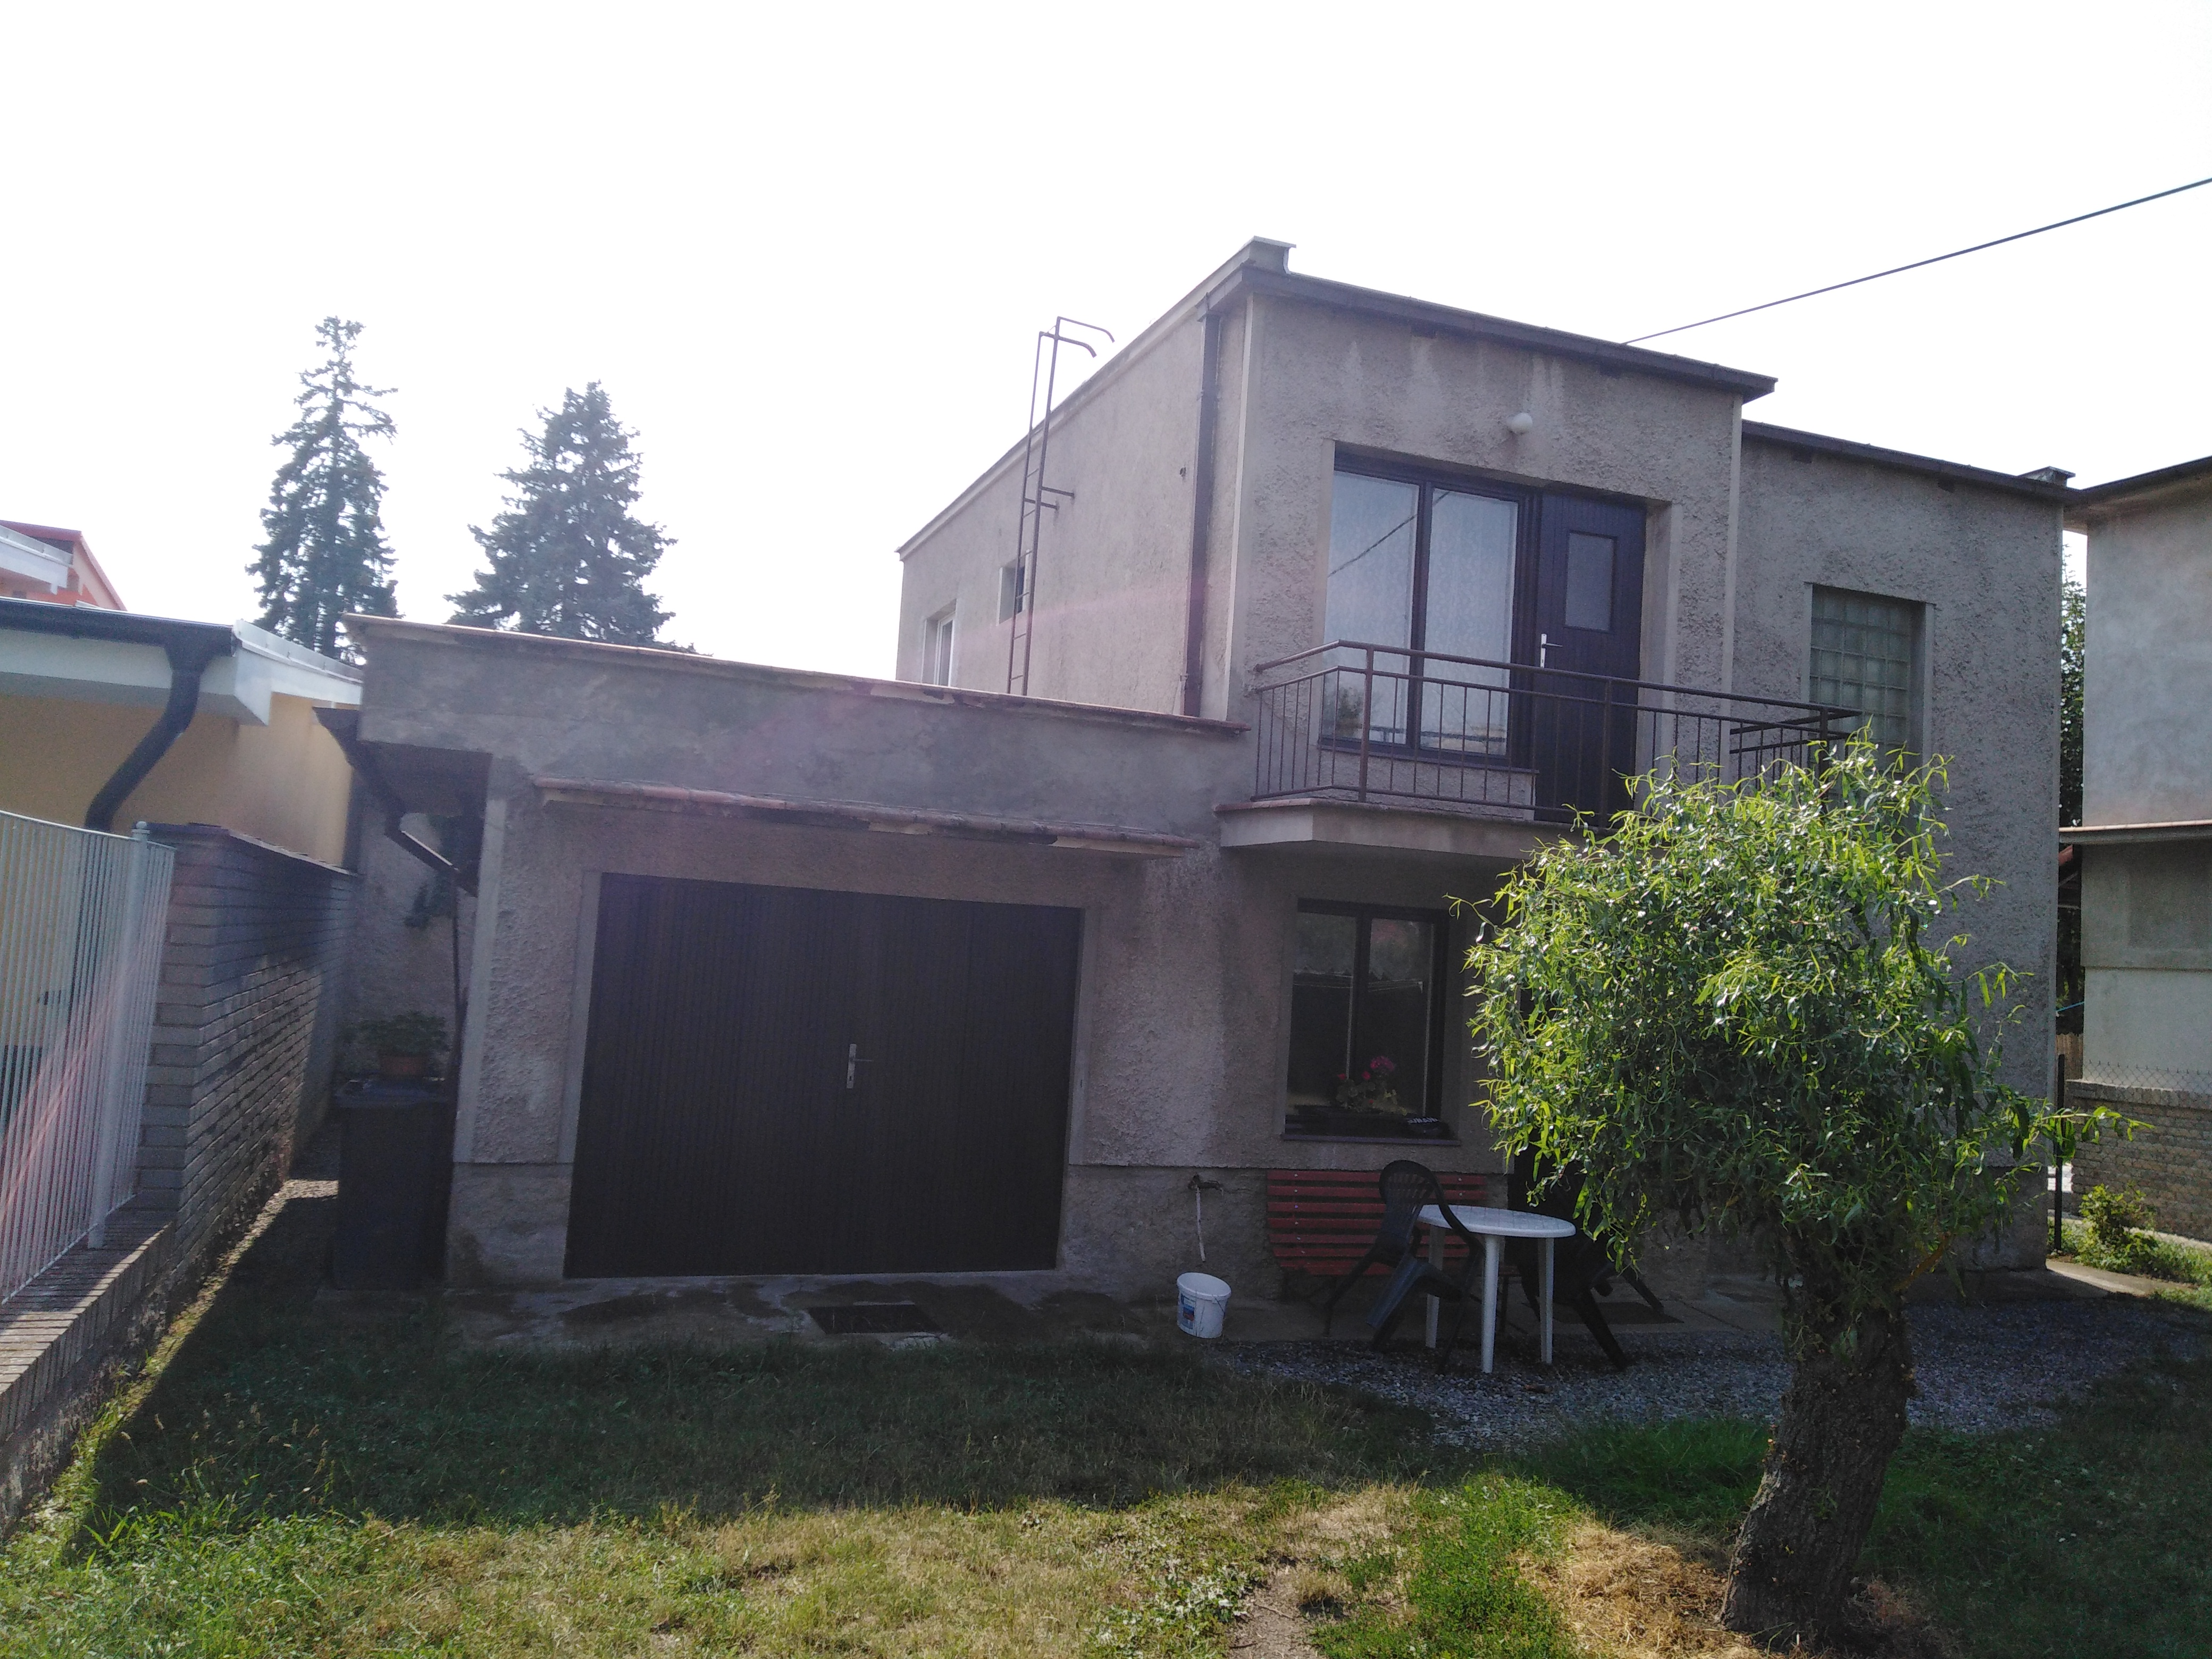
\includegraphics[width=.8\textwidth]{anglicka574/dobrichovice.jpg}
    \caption{Fotografie objektu z přední strany.}
    \label{fig:anglicka574_fotografie}
\end{figure}
\section{Naměřené vývoje OAR, teplot a relativní vlhkosti vzduchu}
\begin{figure}[ht]
    \centering
    \includegraphics[width=1\textwidth]{anglicka574/a1.png}
    \caption{Data z TERA sondy č. 8, která byla umístěna ve sklepě.}
    \label{fig:anglicka574_a1}
\end{figure}
\begin{figure}[ht]
    \centering
    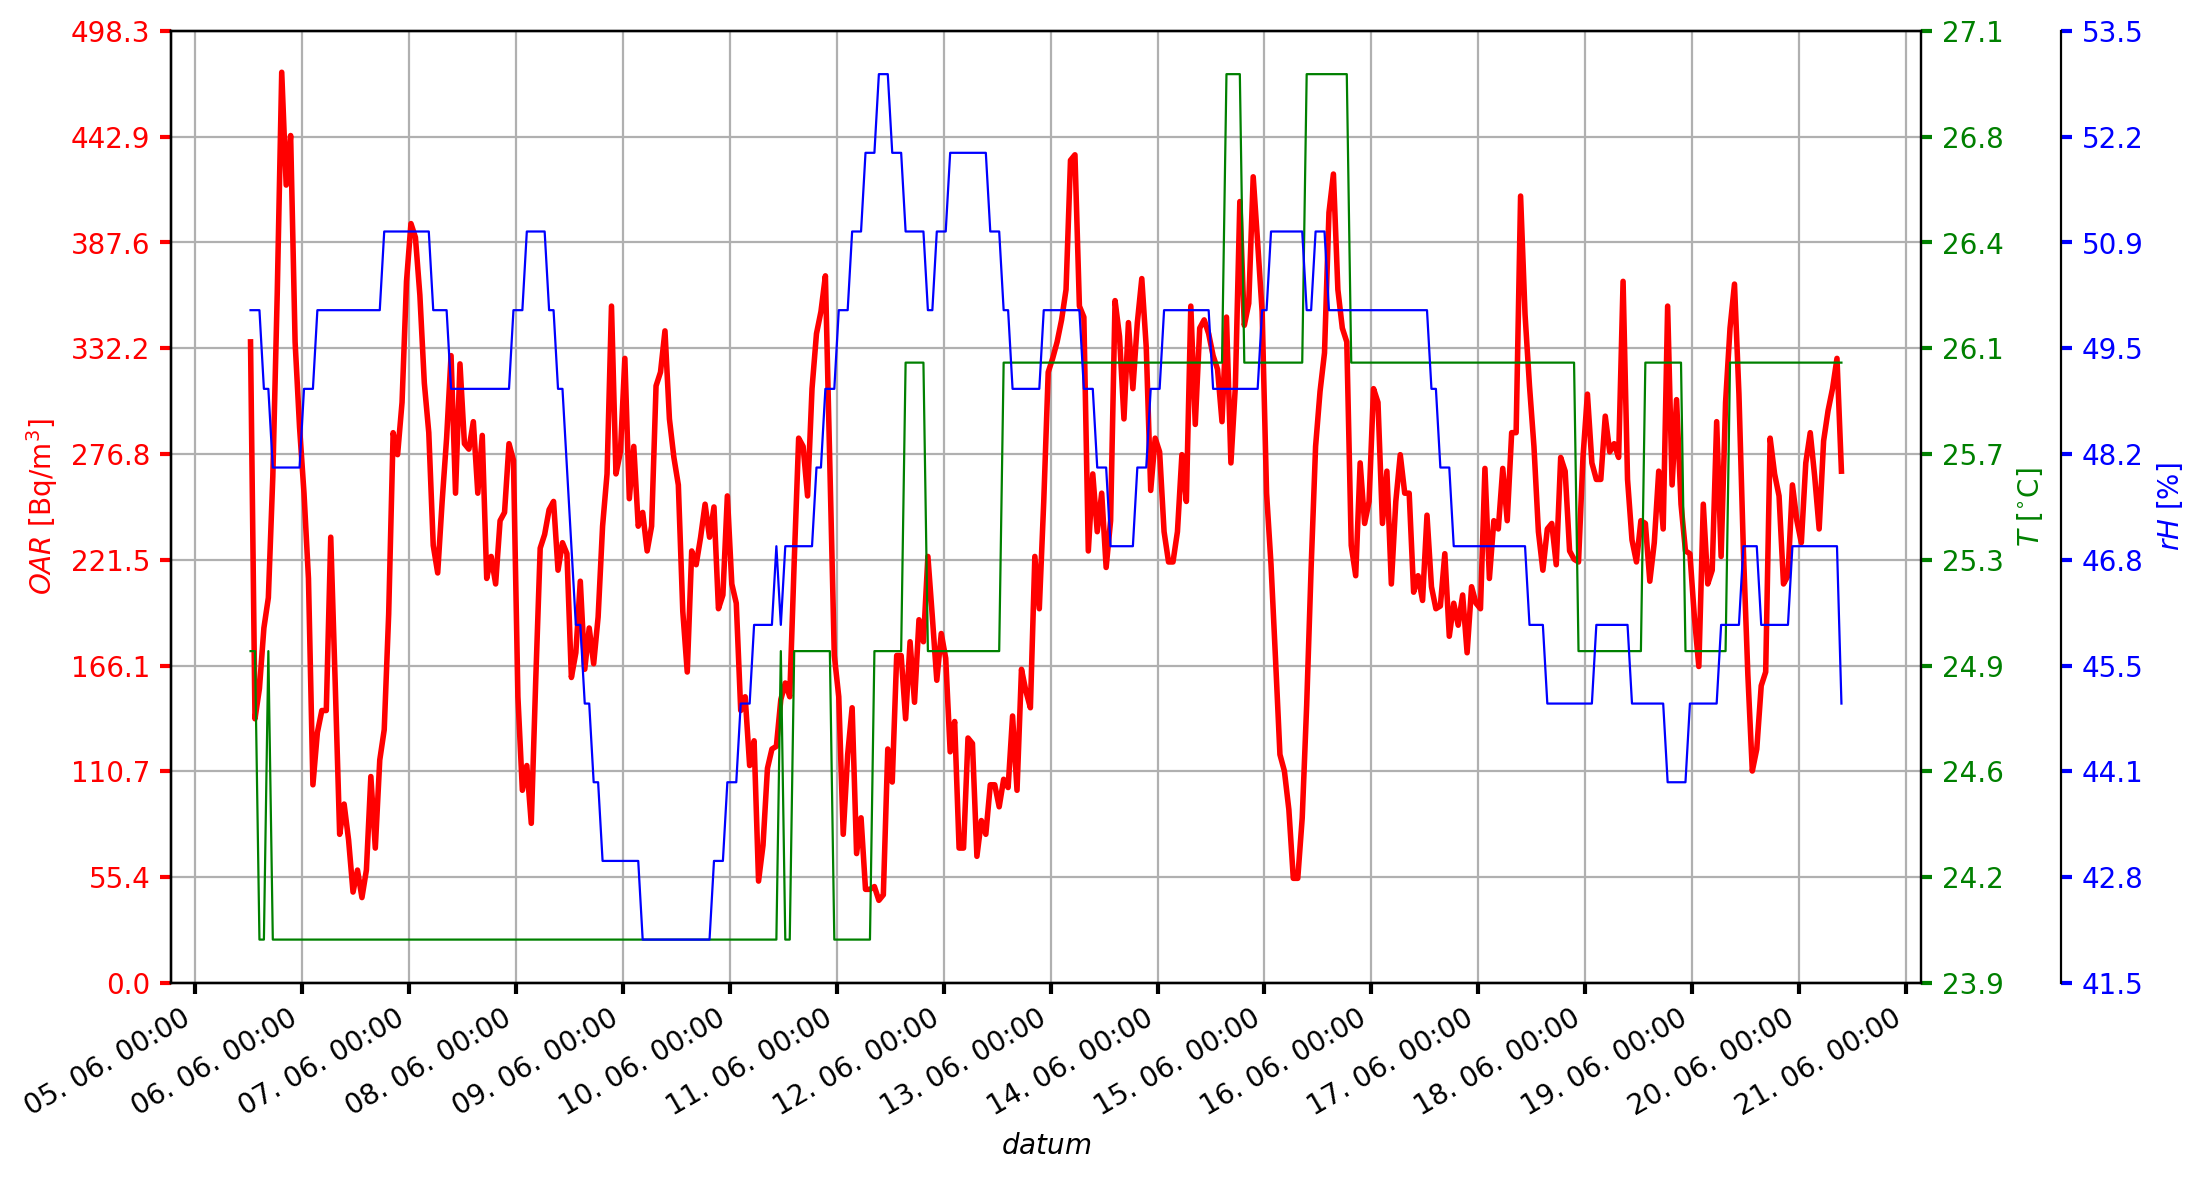
\includegraphics[width=1\textwidth]{anglicka574/a2.png}
    \caption{Data z TERA sondy č. 88, která byla umístěna v přízemí.}
    \label{fig:anglicka574_a2}
\end{figure}
\begin{figure}[ht]
    \centering
    \includegraphics[width=1\textwidth]{anglicka574/a3.png}
    \caption{Data z TERA sondy č. 112, která byla umístěna v prvním patře.}
    \label{fig:anglicka574_a3}
\end{figure}

